\documentclass[10pt, twoside, a4paper,openany]{book}
\usepackage{macra_xelatex}
\usepackage[
backend=biber,
style=ieee,
sorting=none
]{biblatex}
\addbibresource{Chapters/Bibliography.bib}
\usepackage{float}


\begin{document}
% strony generowane z moja.pg
\ifthenelse{\isundefined{\JK}}{
\ifthenelse{\isundefined{\JJ}}{
\ifthenelse{\isundefined{\MM}}{
\ifthenelse{\isundefined{\HL}}{
    
\includepdf{Chapters/Strona_tytulowa.pdf}
}{
    
\includepdf{PerAuthor/StronaTytulowa_193552_HL.pdf}
}
}{
    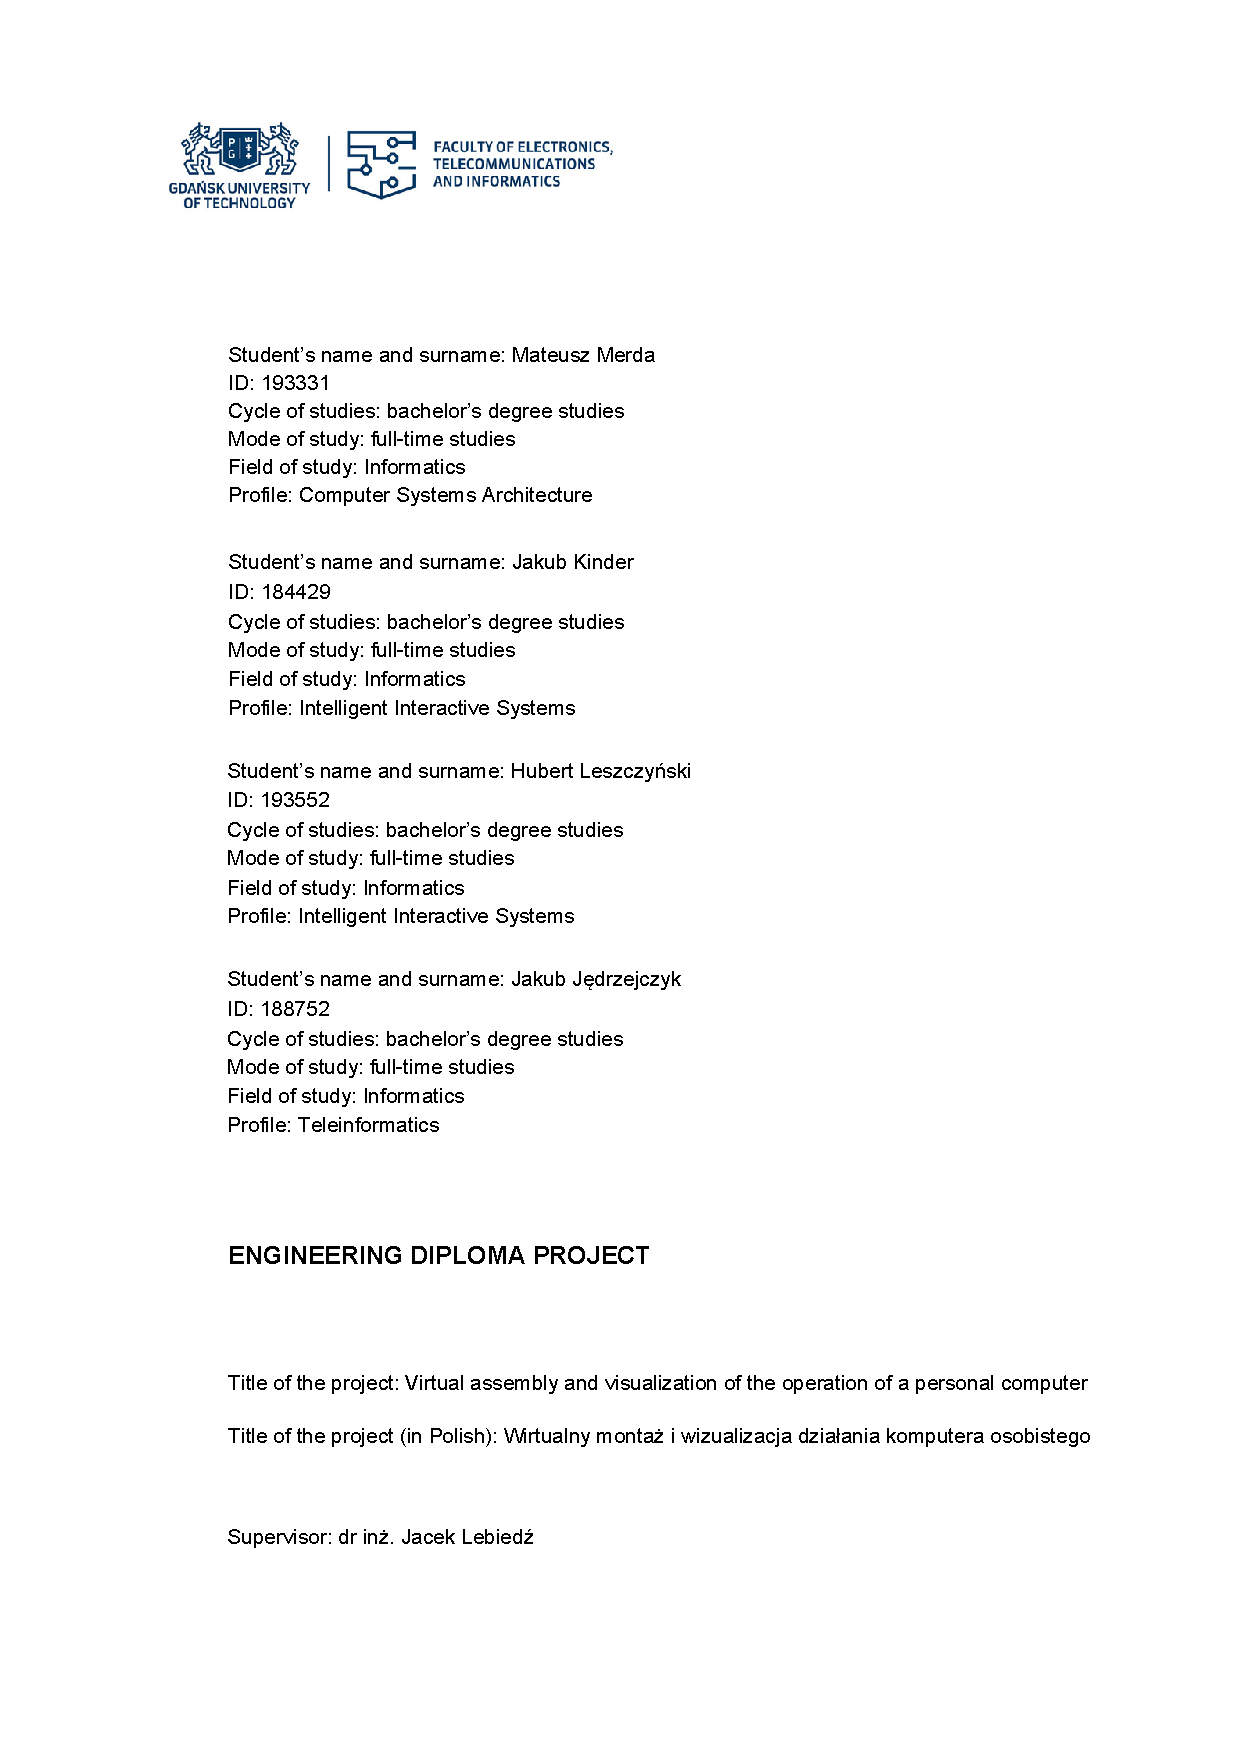
\includepdf{PerAuthor/StronaTytulowa_193331_MM.pdf}
}
}{
    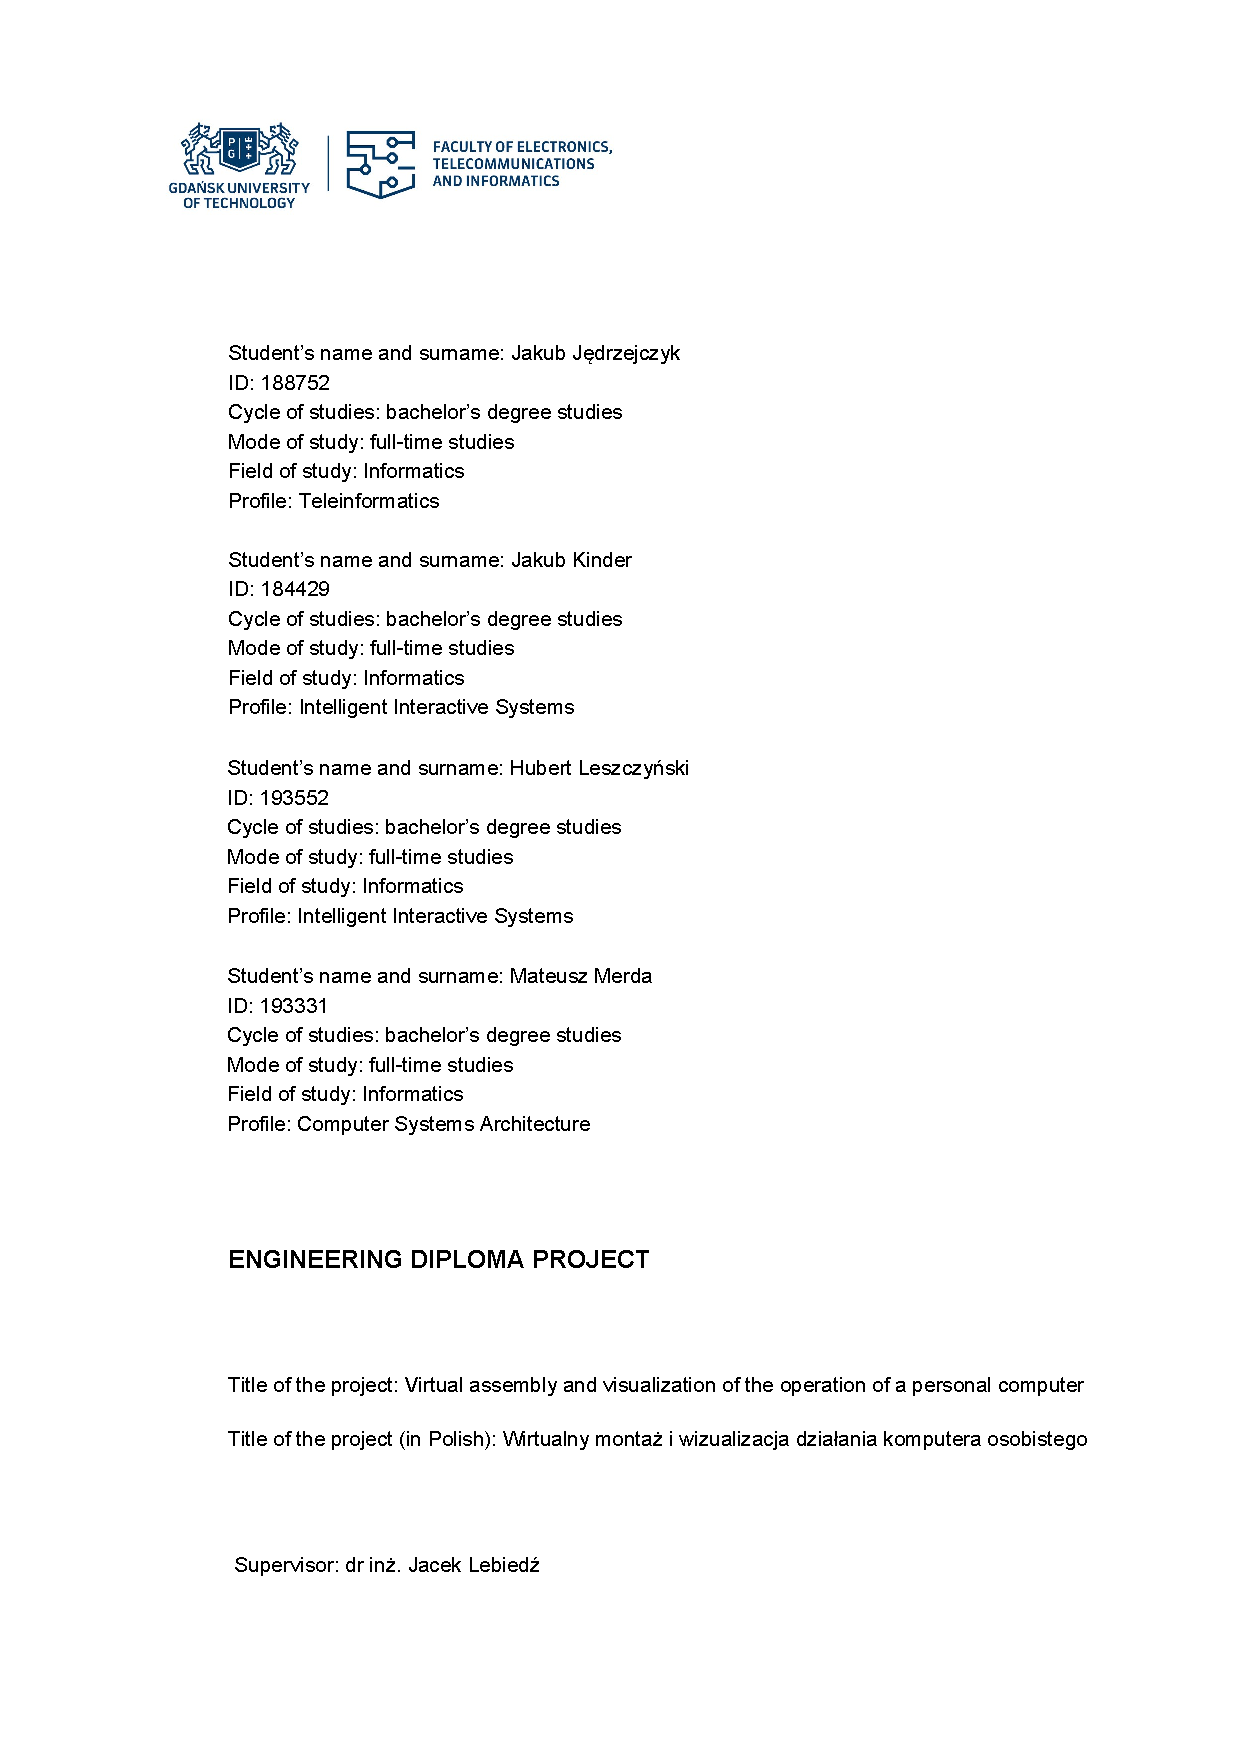
\includepdf{PerAuthor/StronaTytulowa_188752_JJ.pdf}
}
}{
    
\includepdf{PerAuthor/StronaTytulowa_184429_JK.pdf}
}


% streszczenie PL, EN
\chapter*{Streszczenie}
\thispagestyle{plain}

Dzisiejszy rynek podzespołów komputerowych rozwija się w bardzo dynamiczny sposób, co przyczynia się do coraz większej liczby ich możliwych typów, modeli oraz konfiguracji.
Zbudowanie komputera osobistego może więc wydawać się skomplikowanym zadaniem, biorąc pod uwagę kompatybilność sprzętu, a także różnice w budowie poszczególnych podzespołów.
Nauka montażu komputera na rzeczywistym sprzęcie niesie również ryzyko uszkodzenia drogich komponentów, w szczególności podczas montażu delikatnych elementów, takich jak procesor.
Tradycyjne metody nauki, takie jak książki i materiały wideo, nie zapewniają niezbędnej wiedzy oraz praktycznego doświadczenia.
Prowadzi to do rosnącego zapotrzebowania na interaktywne środowisko edukacyjne, pozwalające na naukę budowy komputera bez ponoszenia ryzyka finansowego.
Odpowiedzią na wymienione problemy może być aplikacja wykorzystująca technologię rzeczywistości wirtualnej, wprowadzająca użytkowników w tematykę montażu komputera.

Celem projektu inżynierskiego "Wirtualny montaż i wizualizacja działania komputera osobistego" było zaprojektowanie oraz implementacja wirtualnego trenażera operującego w jaskiniach rzeczywistości wirtualnej, znajdujących się w Laboratorium Zanurzonej Wizualizacji Przestrzennej Politechniki Gdańskiej.
W wyniku prac powstał symulator budowy komputera, oferujący użytkownikom wirtualny montaż licznych konfiguracji sprzętowych, który uwzględnia kompatybilność podzespołów oraz prowadzi ich przez pełen proces w realistyczny sposób.
Aplikacja zapewnia bezpieczne środowisko do nauki budowy komputera, w którym nie występuje ryzyko uszkodzenia drogich komponentów, a możliwość swobodnego powtarzania wykonanych czynności prowadzi do utrwalania nabytej wiedzy.
Wykorzystanie technologii rzeczywistości wirtualnej pozwoliło na dokładne wykrywanie oraz odwzorowanie pozycji rąk i głowy użytkownika, zapewniając mu wysoki poziom immersji w utworzonym środowisku.
W trenażerze zaimplementowane zostały niezbędne mechaniki pełnej kontroli nad podzespołami komputerowymi, pozwalające na ich swobodne przenoszenie oraz łączenie.
Aby zapewnić wsparcie użytkownikowi, utworzone zostały elementy interfejsu aplikacji, które prowadzą go przez każdy etap budowy wirtualnego komputera w przystępny sposób.
Symulator został wytworzony przy użyciu silnika gier Unreal Engine 5, który pozwolił na bezpośrednią współpracę z systemami śledzenia ruchu oraz synchronizacji wieloekranowej projekcji.

Symulator został dokładnie przetestowany w jaskiniach rzeczywistości wirtualnej, a także przeprowadzone zostały badania oceniające jego intuicyjność oraz wartość edukacyjną.
Testy z udziałem użytkowników wykazały ich wysoki poziom satysfakcji, potwierdzając skuteczność trenażera jako narzędzia edukacyjnego.
Dodatkowo przeprowadzono badania porównawcze symulatora z dostępnym na rynku alternatywnym rozwiązaniem, które wykazały zbliżony lub wyższy poziom satysfakcji użytkowników aplikacji rzeczywistości wirtualnej.
Uczestnicy badań pozytywnie ocenili intuicyjność trenażera oraz wykazali większą pewność siebie w zakresie samodzielnego montażu komputera.

Praca inżynierska była realizowana przez zespół czterech studentów.
Każdemu członkowi zespołu przypisane zostały następujące zadania podczas implementacji trenażera oraz realizacji pracy dyplomowej:
\begin{itemize}
    \item \textbf{Jakub Jędrzejczyk} - odpowiadał za zarządzanie zespołem projektowym oraz implementację mechanik kontrolowania podzespołów i montażu komputera oraz za stworzenie czytelnego interfejsu użytkownika. Jest autorem rozdziału \ref{chap:Testing} oraz podrozdziałów \ref{sec:GameEngineSelection}, \ref{chap:GUI}, \ref{chap:ObjectHolding}, \ref{chap:Dtrack}, \ref{chap:ConnectingComponents}, \ref{chap:PCValidation}, \ref{sec:FuturePlans}.
    \item \textbf{Jakub Kinder} - odpowiadał za zaprojektowanie i wytworzenie menedżera procesu budowy komputera, śledzącego jego postęp oraz walidującego utworzoną konfigurację. Jest autorem rozdziałów \ref{chap:Introduction} i \ref{chap:FieldIntroduction}, a także podrozdziałów \ref{chap:buildmanager}. 
    \item \textbf{Hubert Leszczyński} - odpowiadał za zaprojektowanie systemu, dekorację głównej sceny aplikacji, a także wytworzenie trójwymiarowych grafik. Zaimplementował również mechanizm dynamicznego tworzenia podzespołów. Jest autorem rozdziału \ref{chap:project} oraz podrozdziałów \ref{chap:models}, \ref{chap:spawners}, \ref{chap:objectConfig} i \ref{chap:sceneDesign}.
    \item \textbf{Mateusz Merda} - odpowiadał za wytworzenie elementów posiadających zaawansowane konfiguracje fizyki i kolizji. Jest autorem rozdziału 3, a także podrozdziałów \ref{subsec:twohands}, \ref{sec:cableconnector}, \ref{sec:results}, \ref{sec:conclusions}.
\end{itemize}

W przyszłości projekt może zostać rozwinięty o dokładne mechanizmy wizualizacji działania komputera osobistego, a także o większą liczbę dostępnych podzespołów i konfiguracji sprzętowych.
Słowa kluczowe: Rzeczywistość wirtualna, Wytwarzanie aplikacji, Wizualizacja, Budowa komputera
Dziedzina nauki i techniki, zgodnie z wymogami OECD: 1.2 Nauki o komputerach i informatyka
\chapter*{Abstract}

Today's computer component market is developing very dynamically, which leads to an increasing number of their types, models or configurations.
Assembling a personal computer might seem like a complicated task, considering hardware compatibility and differences in the individual components construction.
Learning to assemble a computer on real hardware also carries the risk of damaging expensive components, especially when handling delicate parts such as the processor.
Traditional learning methods, such as books and videos, do not provide the necessary knowledge and practical experience.
This leads to a growing demand for an interactive learning environment that allows users to learn how to build a computer without bearing financial risks.
An application using virtual reality technology, introducing users to the topic of computer assembly, may be the answer to these problems.

The objective of the diploma project "Virtual assembly and visualization of the operation of a personal computer" was to design and implement a virtual trainer operating in the virtual reality caves located at the Immersive 3D Visualization Lab at the Gdańsk University of Technology.
As a result of the work, a computer building simulator was created, offering its users the ability to virtually assemble multiple hardware configurations, taking into account component compatibility, and guiding them through the entire process in a realistic way.
The application provides a safe environment for learning how to build a computer, without bearing the risk of damaging expensive components, and the ability to freely repeat completed steps reinforces acquired knowledge.
The use of virtual reality technology allowed for the accurate detection and mapping of the user's hand and head positions, providing a high level of immersion in the created environment.
The trainer was implemented with the necessary mechanics for full control over computer components, allowing them to be freely moved and connected.
To provide user support, application interface elements were created that guide users through each stage of building a virtual computer in an accessible manner.
The simulator was created using the Unreal Engine 5 game engine, which allows for direct interaction with motion tracking systems and multi-screen projection synchronization.

The simulator was thoroughly tested in virtual reality caves, and a research was conducted to assess its intuitiveness and educational value.
User tests demonstrated high levels of satisfaction, confirming the trainer's effectiveness as an educational tool.
Additionally, comparative research was conducted between the simulator and a commercially available solution, which showed similar or higher levels of user satisfaction with the virtual reality application.
Participants positively assessed the trainer's intuitiveness and demonstrated greater confidence in assembling the computer themselves.

The diploma project was realized by a team of four students.
Each team member was assigned the following tasks during the implementation of the trainer and the diploma thesis completion:
\begin{itemize}
    \item \textbf{Jakub Jędrzejczyk} - was responsible for team management and implementing the mechanics for controlling components and assembling the computer, as well as creating a legible user interface. He authored chapter \ref{chap:Testing}, and sections \ref{sec:GameEngineSelection}, \ref{chap:GUI}, \ref{chap:ObjectHolding}, \ref{chap:Dtrack}, \ref{chap:ConnectingComponents}, \ref{chap:PCValidation}, \ref{sec:FuturePlans}.
    \item \textbf{Jakub Kinder} - was responsible for designing and implementing a build manager, which tracked the progress of the computer assembly and validated the built configuration. He authored chapters \ref{chap:Introduction} and \ref{chap:FieldIntroduction}, and sections \ref{chap:buildmanager}. 
    \item \textbf{Hubert Leszczyński} - was responsible for a system project, designing the main scene of the application, and creating the 3D graphics. He also implemented the mechanic of a dynamic computer component creation. He authored chapter \ref{chap:project} and sections \ref{chap:models}, \ref{chap:spawners}, \ref{chap:objectConfig} and \ref{chap:sceneDesign}.
    \item \textbf{Mateusz Merda} - was responsible for developing objects with advanced physics and collision configurations. He authored chapter 3 and sections \ref{subsec:twohands}, \ref{sec:cableconnector}, \ref{sec:results}, \ref{sec:conclusions}.
\end{itemize}

In the future, the project can be expanded to include precise mechanisms of visualizing the work of a personal computer, as well as a larger number of available hardware components and configurations.
\newline Keywords: Virtual reality, Application development, Visualization, Computer assembly
\newline Field of Science and Technology (OECD classification): 1.2 Computer and information sciences

% spis treści
\tableofcontents

% wykaz skrótów
\chapter*{LIST OF IMPORTANT NOTATIONS AND ABBREVIATIONS}
\addcontentsline{toc}{chapter}{LIST OF IMPORTANT NOTATIONS AND ABBREVIATIONS}


\begin{abbrev}
\item[2D] Two-dimensional - A cartesian space defined by two dimensions, usually marked as X and Y
\item[3D] Three-dimensional - A cartesian space defined by three dimensions, usually marked as X, Y and Z
\item[CAVE] Cave Automatic Virtual Environment - an VR environment, where the immersion is provided to the user through the use of multiple projectors
\item[DLC] Downloadable Content - an additional computer game content, usually downloaded from the internet
\item[GLB] Graphics Library Transmission Binary - a file format used for storing 3D models
\item[GUI] Graphical User Interface - a type of an user interface, which provides the user a possibility to interact with the computer by using multiple graphical assets
\item[MoSCoW] Must, Should, Could, Won't - A scale for determining the priotities of a project's requirements
\item[OOP] Object-Oriented Programming - a programming paradigm focused on the conception of objects, that can interact with each other
\item[PC] Personal Computer - A multipurpose device designed for an user's personal operation
\item[UE5] Unreal Engine 5 - A game engine developed by Epic Games company
\item[UI] User Interface - a mechanism that allows the user to interact with the computer
\item[UML] Unified Modeling Language - a language used for creating multipurpose models
\item[VR] Virtual Reality - a technology providing the user with immersion in a simulated 3D environment by using specialized equipment
\end{abbrev}



% rozdziały i podrozdziały numerowane
\chapter{INTRODUCTION (Jakub Kinder)}
\label{chap:wstep}

Nowadays, building a PC is becoming increasingly popular due to its capability to address users' personal requirements towards the device.
% ^ truizm, z którym się zgadzam, ale dobre by było źródło
However, with this rise in interest, the knowledge and skills regarding computer assembly were not spread alongside it.
% ^ nie wiem czy się z tym zgadzam, ale jest to co najmniej mocna teza
To this day, this leaves many people helpless when it comes to building their own PC from scratch. 
It also stands to reason that people with little to no knowledge on the subject do not try their hands at assembling PCs.
The main cause of it is the cost of parts needed for a fully functional PC and the fact that they tend to be delicate, especially the connection pins on components such as GPU or CPU, which happen to be the most expensive parts.
Hence, many tools and applications were developed to aid people in this endeavor.
Most of these tools focus on helping users pick adequate components for their new PC without accounting for their size compatibility, placement, or installation process.
% ^ to jest niewygodne stwierdzenie biorąc pod uwagę, że istnieją aplikacje takie jak PCPartPicker, które sprawdzają kompatybilność części - są nawet wspomniane w dalszej częsci pracy
For these reasons, some game developers and studios created simulation games that address those issues, with differing levels of overall quality.
% ^ oryginalnie było "that solve those issues" - gdyby rozwiązywały problemy, to nie mielibyśmy po co pisać tej pracy, także trzeba było to zmienić
The most popular and advanced of such simulators is PC Building Simulator \cite{pcbuilder}.
% ^ spacja przed cytowaniem być musi

With the development of Virtual Reality (VR), a whole new environment for games and applications was created.
Plenty have taken this opportunity to create incredibly immersive simulations that were not possible in a traditional 3D setting and pioneered this field, pushing the capabilities of this newly developed technology.
% ^ przydałyby się przykłady (np. Half-Life: Alyx, Boneworks, Microsoft Flight Simulator VR, itp.)
Even now, true boundaries of VR seem undefined, which leaves plenty of room for new genres and fields to be created or explored.
% ^ można pokazać że granice są dalej przesuwane i podać jakieś przykłady, albo podać różne przykłady w jaki sposób się przesuwają (haptyczne kontrolery, lepsze headsety (BigScreen Beyond 2, Apple Vision Pro))

In recent years, many VR games have been made in that genre, and all of them feature much greater immersion than their regular 3D counterparts, despite the fact that they possess superior graphic solutions.
% ^ może ja jestem niezbyt sprytny, ale "that genre" wydaje mi się być niejasne - o jaki gatunek chodzi?
% oprócz tego "superior graphic solutions" jest powierzchownym potraktowaniem tematu - gry VR muszą renderować dwa widoki dla obu oczu co znacznie zwiększa rozdzielczość
Moreover, currently sold, ready-to-use PCs are often far more than capable of running VR applications, and the cost of obtaining appropriate equipment consisting of a specialized headset and hand controllers is decreasing.
However, despite these changes, till this day no one has released a VR PC building simulator of any kind.

The goal of this project is to fill the aforementioned void in VR simulation games, by designing and implementing a PC building simulator in a VR environment.
Such a solution will feature far greater immersion than its 3D, non-VR counterparts.
% ^ "3D" może też technicznie oznaczać VR, ewentualnie "traditional 3D"
Also, it would create a possibility for the spread of both knowledge and skills in this area.
Additionally, the developed application will allow users to test the configuration of components and their ability to assemble it in a timely manner. 
However, the most important area of this application will be the introduction to the complexity of building a PC, ranging from its construction, through the installation process of all its essential components, to the verification of its functionality and expected performance.
% ^ trochę rozszerzyłem to zdanie, żeby brzmiało bardziej jak "duży cel", ale przydałoby się też określenie jakie wartości (edukacyjne) może to nieść

% dodatkowe propozycje:
% - paragraf o tym dlaczego akurat istniejące symulatory nas nie zadowalają (nie w niesamowitych detalach, ale jakieś ogólne punkty)
% - dodatkowe określenie docelowej grupy użytkowników
% - krótkie wspomnienie o tym, że aplikacja jest technicznie możliwa dzięki postępowi technologicznemu w dziedzinie VR
\chapter{FIELD INTRODUCTION (Jakub Kinder)}
\label{chap:FieldIntroduction}

The main goal of this chapter is to present current information about PC building and its market.
It consists of descriptions of components and their compatibility, the assembly process as well as the most popular tools used to aid people both novice and experienced in the field.
However, it also explores currently available simulators, and how advanced and precise they are.
Another topic of this chapter is how VR as an environment is used and what advantages it has in the context of hardware assembly and visualization.

\section{PC building}
Nowadays, computers are built using modular components, which simplifies their construction and allows for immense flexibility regarding choice of components.
However, as mentioned in \autoref{chap:Introduction}, PC building still requires comprehensive knowledge not only about the process itself, but also the parts, their ports and physical dimensions.

\subsection{Components, ports and compatibility}
Every single component used in PC building possesses either a port, socket or connector with specific version or standard, which dictates compatibility with other components.
Furthermore, some parts have even stricter rules, requiring specific parametric matching to ensure proper function and physical fit within the enclosure.

\subsubsection{CPU}
Commonly known as the brain of a PC, the CPU is connected to a dedicated socket on the motherboard.
Compatibility is fundamentally spit across to manufacturers, Intel and AMD, which utilize incompatible connections standards.
Intel uses Land Grid Array (LGA), while AMD uses Pin Grid Array (PGA) or derived technology.
In addition, both types have their versions and sets of supported architectures, which means not every CPU will fit the same socket even if the type and version is matched.

Critical compatibility parameters:
\begin{itemize}
	\item Socket type: As mentioned above, For CPU to be compatible with a motherboard, the socket must match CPU's type, version and architecture.
	\item RAM controller limit: CPUs can support only specified amount of RAM, number of channels and RAM module's frequencies.
\end{itemize}

\subsubsection{RAM}
This component serves as system's primary volatile storage.
Its compatibility is perhaps the most nuanced of all parts used in PC building, as it is not only limited by CPU, but also RAM module's physical dimensions are a major factor in its compatibility with other components.
In addition, RAM uses Double Data Rate Synchronous Dynamic Random-Access Memory (DDR SDRAM or commonly referred to as DDR) technology, which uses Dual In-Line Memory Module (DIMM) slots.

Critical compatibility parameters:
\begin{itemize}
	\item Generation: Currently there are several generations of DDR available, most recent are DDR4 and DDR5. 
	Unfortunately, DDR technology is not compatible across its generations, so if port utilizes DDR4, RAM of no other generation can be installed in it, as is stated in Micron Technology's article \cite{noauthor_whats_2025}.
	\item RAM frequency: This aspect is the reason why RAM is considered one of the more nuanced components. 
	As mentioned earlier, CPU can support only specified values of this parameter, but the range of accepted frequencies is also limited by the motherboard, which also supports only specified values.
	In addition, all installed sticks of RAM must have the same value of this parameter, however, unlike CPU, they do not have the manufacturer constraint.
\end{itemize}

\subsubsection{GPU}
A specialized piece of hardware responsible for rendering graphics, which is more often than not, a critical component in most PCs.
It utilizes Peripheral Component Interconnect Express (PCIe) x16 interface for connection with the motherboard.
Unlike previously mentioned CPU sockets or RAM slots, PCIe is forwards and backwards compatible standard as is stated in Intel's article titled "What Are PCIe 4.0 and 5.0?" \cite{noauthor_what_nodate}.
This means that GPU with currently the newest PCIe version 5 can be connected to a version 4 slot and vice versa.
The only drawback with such connection is loss of performance, due to lower bandwidth on the side with lower version.

\subsubsection{Memory drive}
This component is usually either a Solid State Drive (SSD) or Hard Disk Drive (HDD), regardless of the type, its purpose is to store data long term.
The main differences between the two types are read/write speeds, in which SSDs are superior, and total amount of storage, which HDDs excel at.
Despite their differences, both types of memory drives utilize the same connection standard, Serial Advanced Technology Attachment (SATA).
Currently, there are three versions of this standard, SATA I, SATA II and SATA III, and just like PCIe, this standard is backwards compatible, with the drawback being drop of bandwidth to that of the lower standard. \cite{noauthor_what_2023}
Additionally, there is another type of memory drive called Non-Volatile Memory Express (NVMe), which instead of SATA, uses M.2, a PCIe x4 interface form factor.
These drives have even higher read/write speeds than regular SSDs, while offering similar amount of storage with the drawbacks being slightly shorter lifespan of the drive and the fact that not all motherboards have PCIe x4 slots.

\subsubsection{Motherboard}
This is the most crucial component in terms of compatibility, because every component mentioned above connects to it.
The motherboard determines, which CPUs, RAM modules, and memory drives can be installed.
Another important aspect for the motherboard is its form factor, the physical dimensions of the component.
The most common standard is Advanced Technology Extended (ATX), which states that motherboard should be 305 x 244 mm.
However, there are smaller standards like mini- Information Technology Extended (ITX) with dimensions of 170 x 170 mm.

Critical compatibility parameters:
\begin{itemize}
	\item CPU socket: As mentioned in CPU's compatibility, the connected CPU's connector must match the socket as well as CPU's architecture must be included in supported list of architectures of the motherboard.
	\item RAM: In this case compatibility is the most complicated as it was stated in RAM description. 
	Not only RAM modules must meet previously discussed requirements, but also they should be included in Qualified Vendor List (QVL) of the particular motherboard.
	\item Form factor: Motherboard's size, critically affects how other components are compatible with it on a more physical level, with ATX standard there might not be any issues, however, mini-ITX offers far less space which can prove problematic for components like RAM modules or GPUs.

\end{itemize}

\subsubsection{Power supply}
Power supply as the name suggests provides power to all the other components, which makes determining its compatibility straightforward.
It must deliver enough power to the computer, but while condition is simple it is one of the most important ones as not meeting it might result in damaging other components caused by improper function due to lack of power.

\subsection{The process of PC assembly}
Due to modular design of modern day computers, assembly in itself is straightforward, but still requires caution as some components require counterintuitive strength to be installed.
Most books and guides such as "Montaż komputera {PC}. {Ilustrowany} przewodnik" \cite{chabinski_montaz_2012} or Intel's guide on PC building \cite{noauthor_how_nodate} agree on general procedure of PC assembly, which is as follows:

\begin{enumerate}
	\item Before the actual assembly procedure, the case, that is to be used in the process must be prepared by removing its side and often front panels as well as screwing in separators on which the motherboard will be mounted.
	\item The first step of the building process is to install the CPU in the dedicated socket on the motherboard.
	It is done by opening the latch on the socket and very gently dropping CPU into it, followed by closing the opened latch.
	\item Optionally, after installing the CPU, NVMe drive can be installed if the motherboard possesses an M.2 slot.
	\item Next is to install RAM, first latches need to be unlocked on both sides of slots pointed out by motherboard's manual.
	Then, RAM modules are to be inserted into the slots, this operation requires counterintuitive amounts of force, thus prior to applying it, one must make sure that the modules are properly oriented, so as not to damage them or the slots.
	\item Afterward, the most common practice is to mount the power supply in previously prepared case, which is done according to case's manual.
	\item Subsequently, the partially assembled motherboard is to be installed in the case, be gentling placing it on the separators and screwing it in. 
	\item Next, the GPU must be installed, which is done by simply inserting it into the PCIe x16 slot on the motherboard and securing the component to the case using provided screws.
	\item The last components to be installed are the memory drives, if M.2 drives were already installed this step is optional.
	It is done be mounting the SSD or HDD drives in spots pointed out by the case manual, followed by connecting SATA cables to bot the drives and the ports on the motherboard.
	\item The final step of the assembly is to connect the power supply cables to the appropriate slots on other components, as well as connect smaller connectors leading from some components to the motherboard.
	These should be attached according to manuals of each component and the schematic included with the motherboard.
\end{enumerate}

\section{PC building market}
In recent years, PC building has become increasingly popular, majorly due to people's demand for customized and potentially more powerful devices.
For this reason, sales of PC parts have skyrocketed and so did the selection of purchasable components. 
According to most of the accessible reports on the PC parts market, like the report from PMarketResearch \cite{article} from the end of 2023, the gaming PC market alone was valued at approximately 18 billion USD and is expected to grow to around 200 billion USD by 2034.
Additionally, most recent and specific market reports are valued at 3,000 USD per copy.
Those facts show that the PC parts market is extremely volatile and rapidly expanding, so much so that just information on it is highly profitable.

\subsection{Existing PC building support tools}
The aforementioned rapid growth of the PC parts market is a direct result of heightened interest in PC building, which for years now has been supported by web applications that help choose compatible parts for a new machine.

\begin{enumerate}
    \item PCPartPicker \cite{PCPartPicker}
    
PCPartPicker is a popular tool for those interested in PC building. 
Its main features are simplified mechanic of choosing components and automatic compatibility guide which supports user in choosing proper components for their future machine. 
This solution also features categorized, sortable lists of components to limit the chance of providing too many choices at once.
The build page's main interface is presented on Figure \ref{fig:partpicker}.

\begin{figure}[!ht]
	\centering
	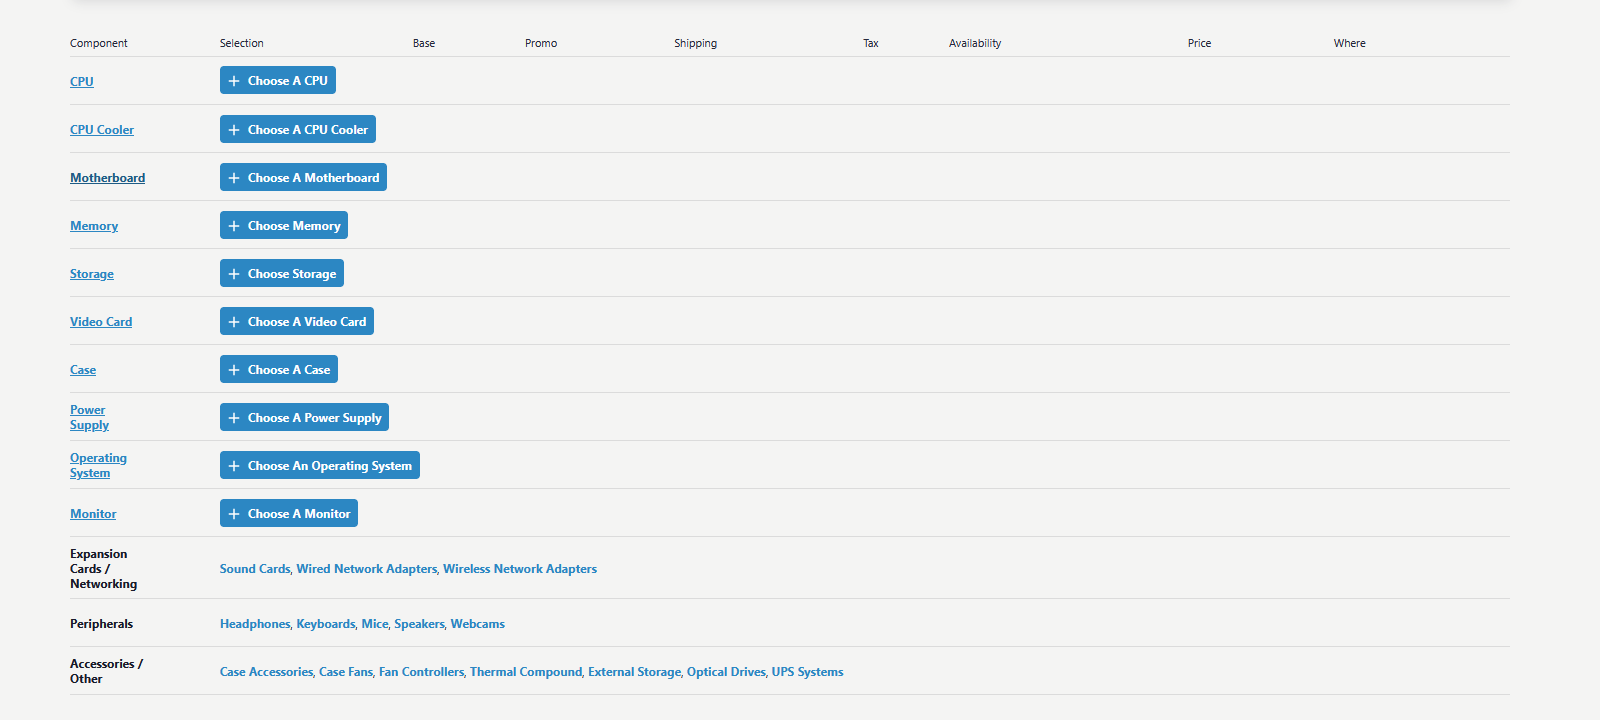
\includegraphics[width=0.6\textwidth]{Images/PCPartPicker.png}
	\caption{Screenshot of PCPartPicker.com build page}
	\label{fig:partpicker}
    \end{figure}

    \item BuildMyPC.net

This tool boasts itself on its simplicity, and while it accomplishes that it still overloads unexperienced users. 
It does it mainly through use of uncommon names of parts and including less used parts like network adapters, which usually are part of motherboards.
Those issues are shown on BuildMyPC.net's build page on Figures \ref{fig:buildmypc1} and \ref{fig:buildmypc2}
Aside from such a shortcoming, it remains as a popular aid tool for choosing a set of compatible PC parts.

\begin{figure}[h!]%
	\centering
	\subfigure[]{
		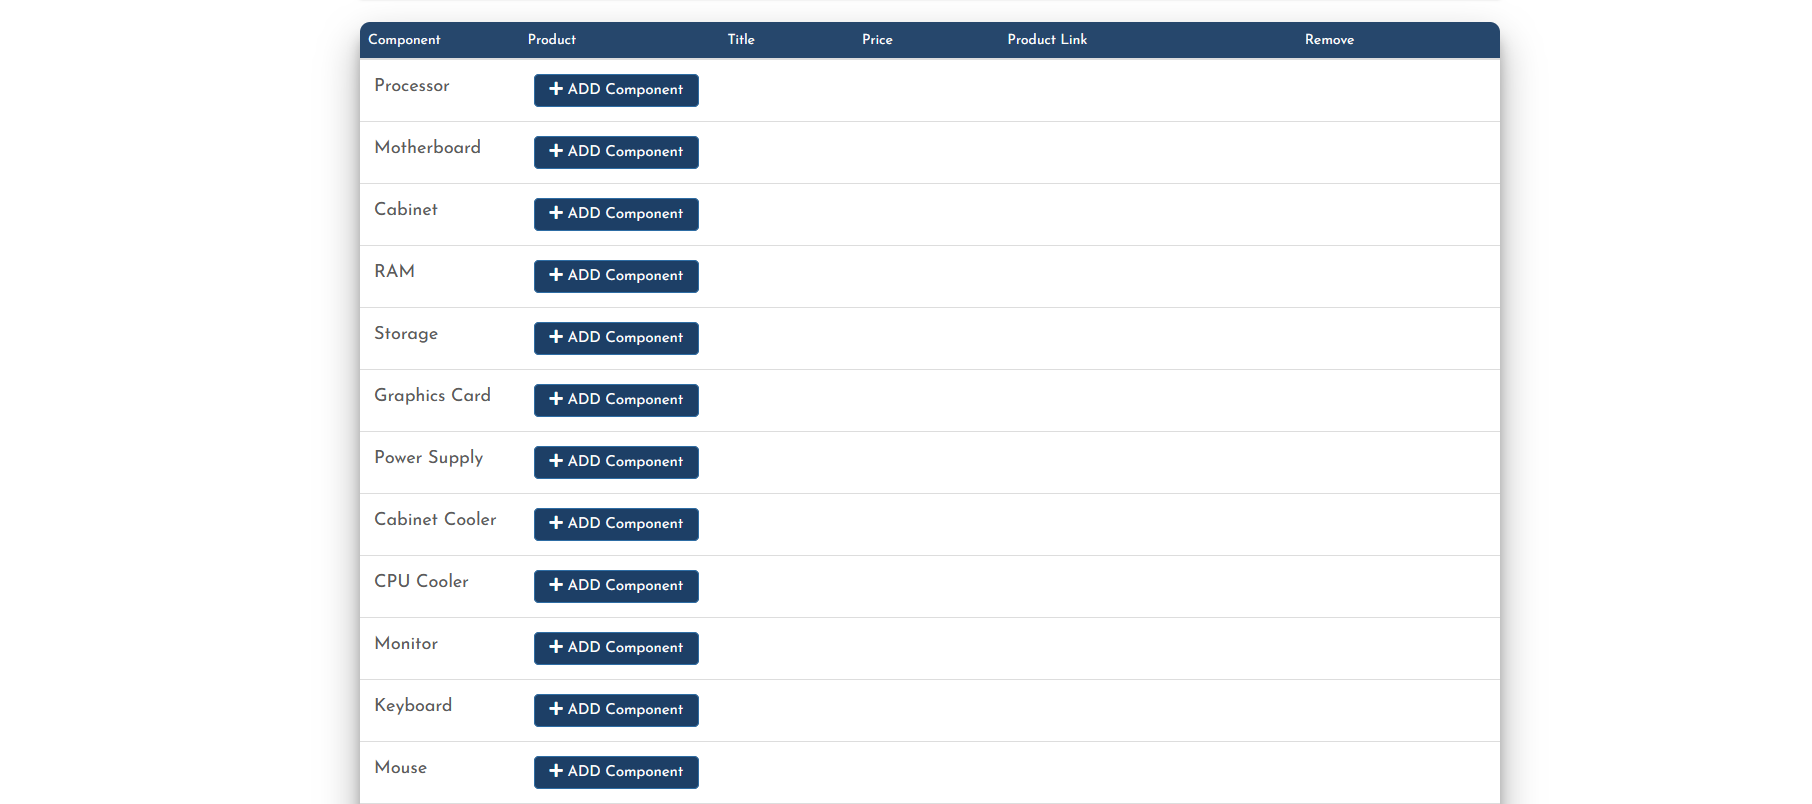
\includegraphics[width=0.48\textwidth]{Images/BuildMyPC.net1.png}
		\label{fig:buildmypc1}
	}%
	\hfil
	\subfigure[]{
		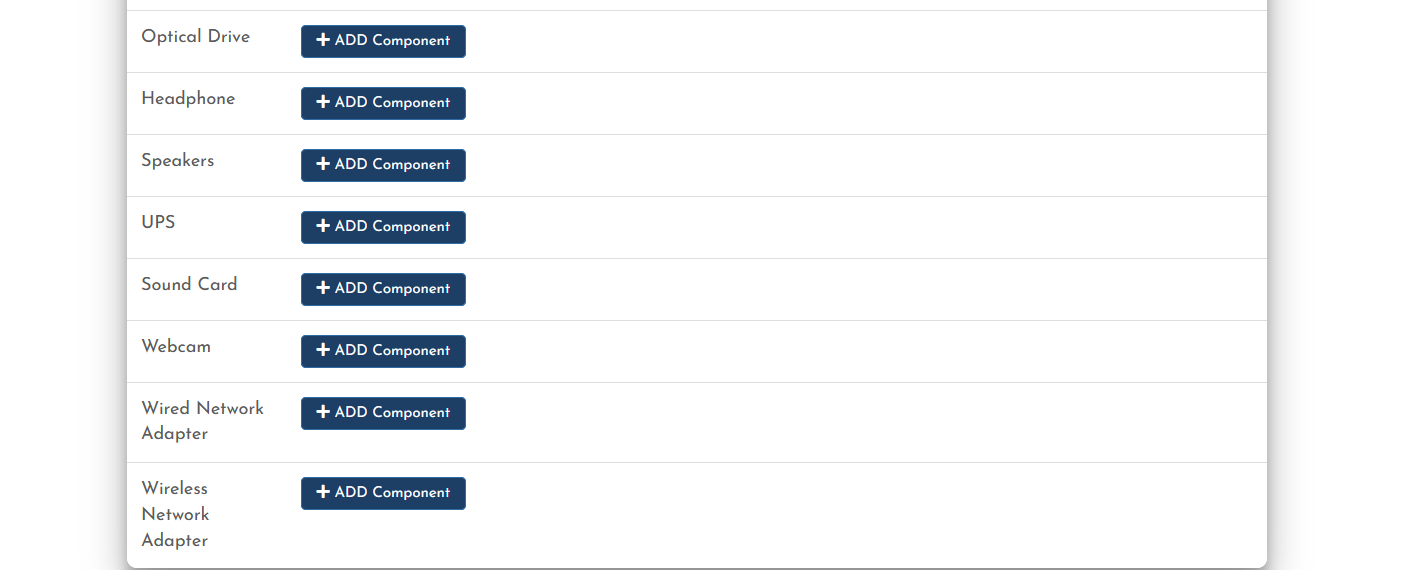
\includegraphics[width=0.48\textwidth]{Images/BuildMyPC.net2.png}
		\label{fig:buildmypc2}
	}
	\caption{Screenshots of BuildMyPC.net build page}
\end{figure}

    \item Logical Increments

    This item is a ranked list of PC parts which helps people choose  relatively up-to-date components to prolong longevity of newly built devices.
    The list consists of 16 ranks for each major PC part, like GPU, CPU, motherboard, SSD or HDD storage etc.
    Whats worth noting, is that each component is placed on the list based on many factors, mainly its based on components parameters but as it stands, the price also plays a major role in component's final placement. 
    Figure \ref{fig:logicalinstruments} presents small piece of mentioned list, and its notable feature is that each rank's sub-list can be further extended to view more parts. 

\begin{figure}[!ht]
	\centering
		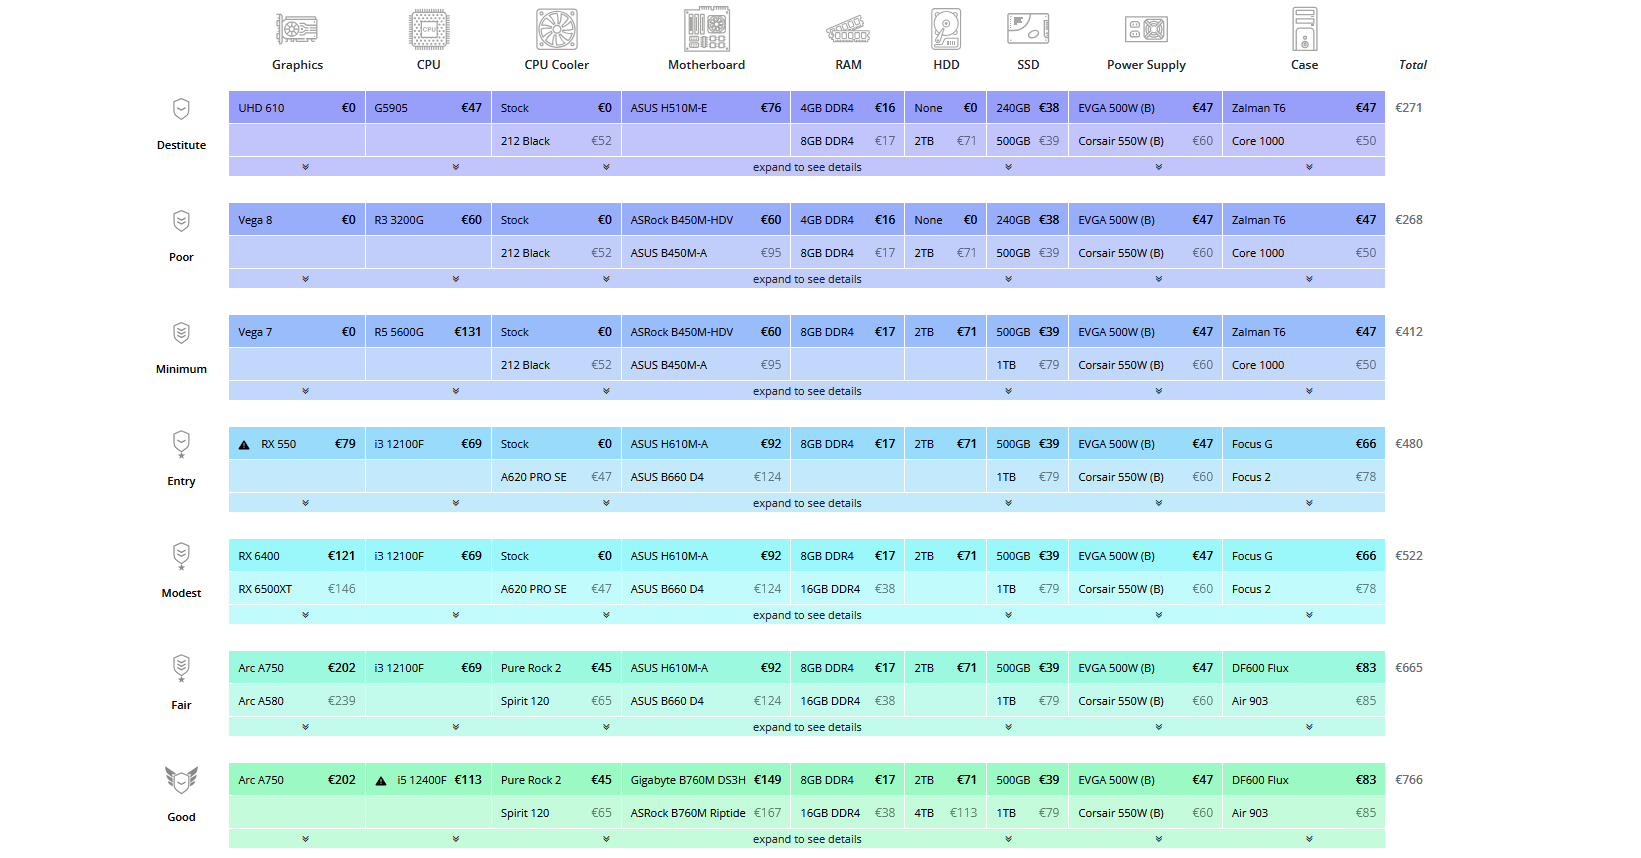
\includegraphics[width=0.85\textwidth]{Images/Logical_Instruments.png}
	\caption{Screenshot of a piece of Logical Instruments ranked list}
	\label{fig:logicalinstruments}
    \end{figure}
    
    \item PC Builder

This tool, while almost identical to PCPartPicker, features a more user friendly interface, ranging from visuals to phrasing of more specialized accessories, like thermal paste.
Its appearence can be observed on Figure \ref{fig:pcbuilder}.


\begin{figure}[!ht]
	\centering
		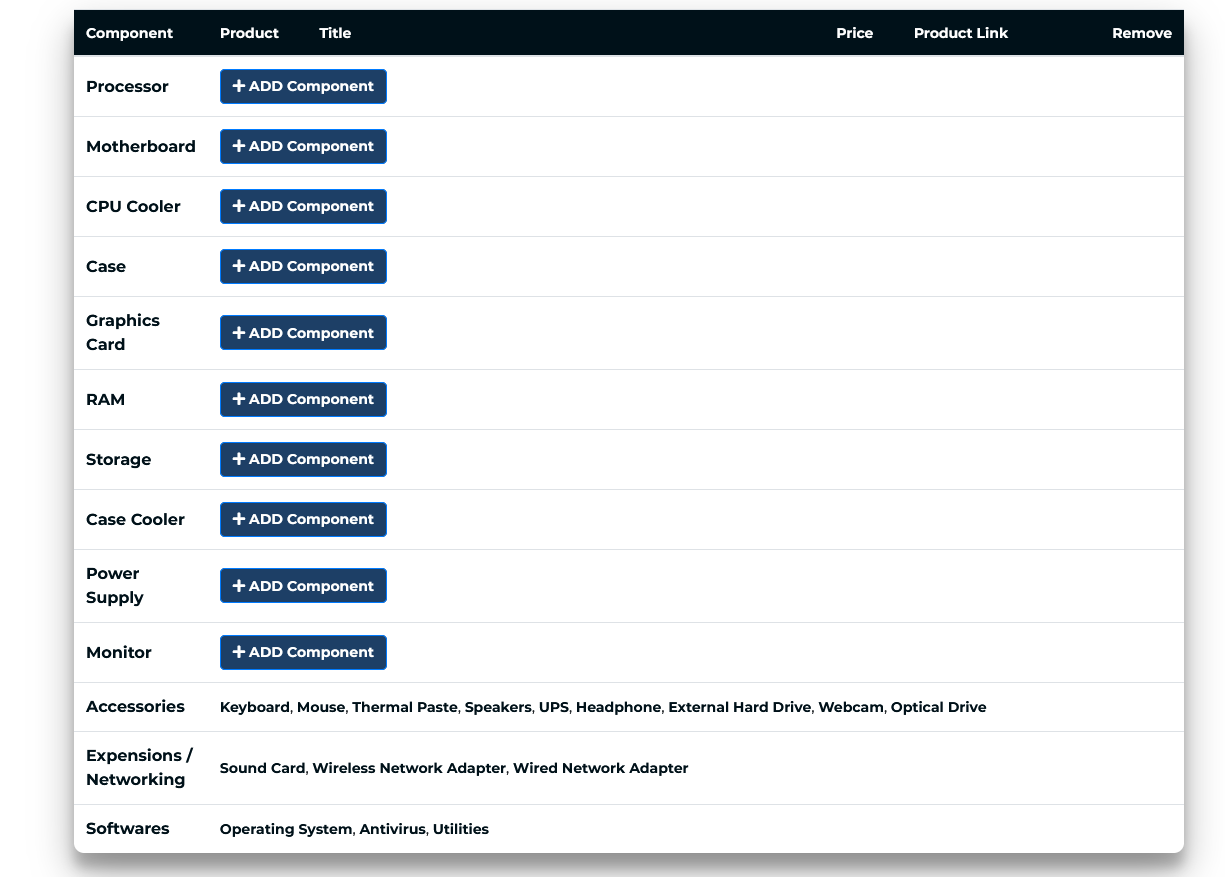
\includegraphics[width=0.7\textwidth]{Images/PCBuilder.png}
	\caption{Screenshot of a configuration component of pcbuilder.net website}
	\label{fig:pcbuilder}
    \end{figure}
    
    \item UserBenchmark

It is a comprehensive collection of over 350 million benchmarks of over 2 million unique components.
Additionally the website features a custom software for testing already built PC to check how well they will perform under current standards.
Other interesting features are, a compare module which allows uses to compare various components of given type and the other is voting system which allows users to rank specific components.
Aforementioned features can be observed on Figure \ref{fig:userbenchmark}.

\begin{figure}[!ht]
	\centering
		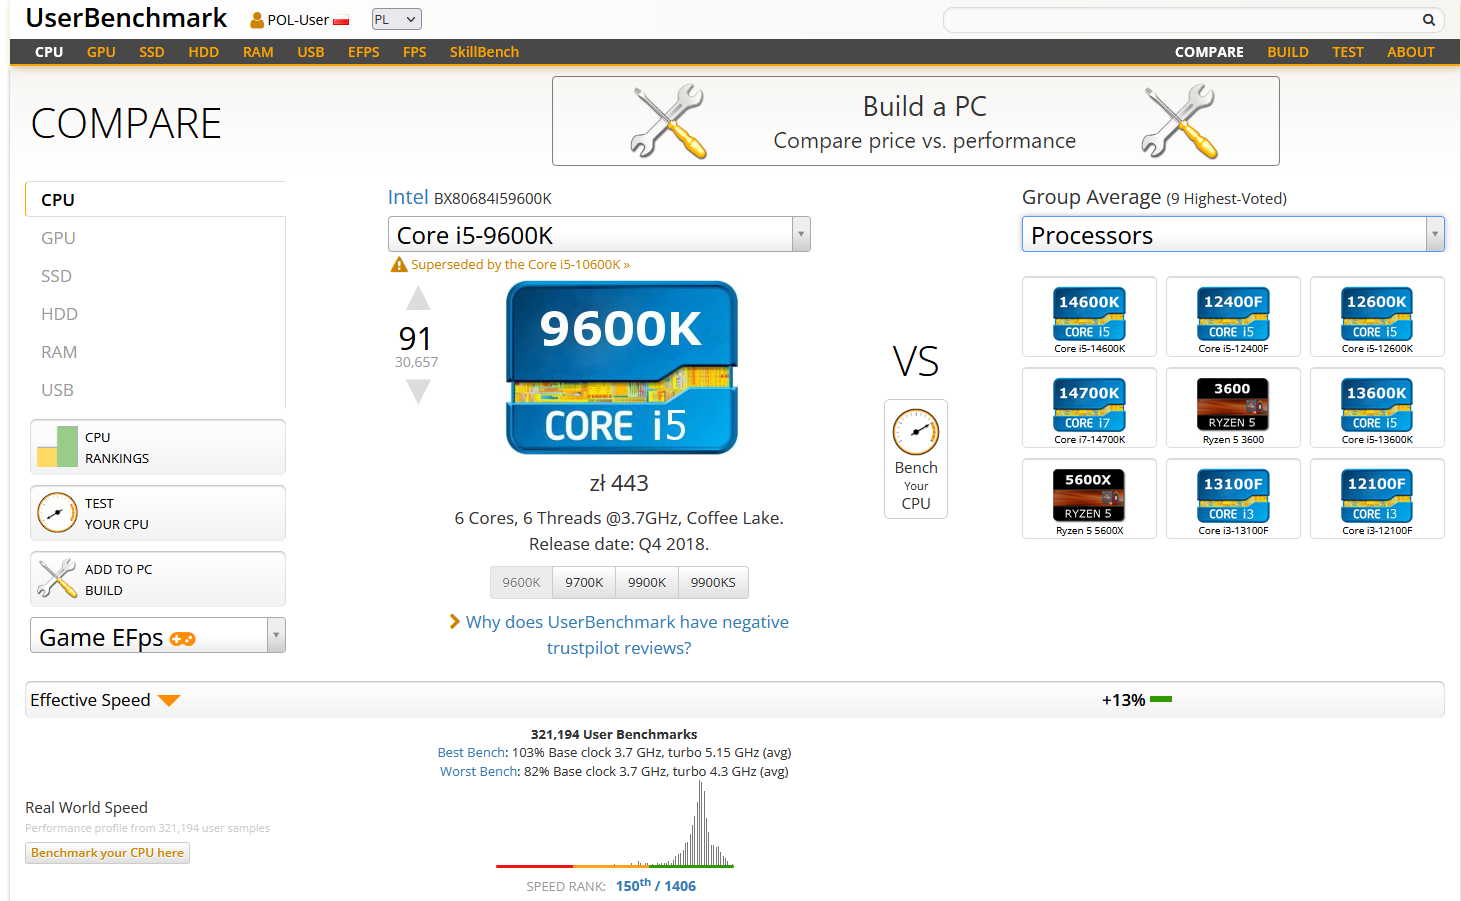
\includegraphics[width=0.7\textwidth]{Images/UserBenchmark.png}
	\caption{Screenshot of a UserBenchmark's CPU compare module}
	\label{fig:userbenchmark}
    \end{figure}
    
\end{enumerate}

\subsection{PC building simulators}
The market of PC building simulators is very limited when it comes to options.
In the desktop section alone, there are only 2 simulators, both from the same authors and in the same franchise.
Such circumstances make it hard to find an appropriate amount of material to base a new simulator on.
However, present options are comprehensive enough to satisfy the market, at least for simulators in a traditional 3D environment.

    \subsubsection{PC Building Simulator 1}
    
Released on 29th January 2019, PC Building Simulator 1 is a simulation game that pioneered PC building simulations in a 3D environment.
Before its release, the only tools used for aid in pc building were configuration apps, guides, and articles on the topic.
However, this game revolutionized the field by introducing actual 3D rendering of the components and featuring a simplified yet still realistic assembly process.

Apart from its origins, it is well known for its wide variety of rather realistically made PC part models.
Not only that, but this game features licensing from component manufacturers like Intel, AMD, NVIDIA, Corsair, and many others.
Figure \ref{fig:pcbspartners} presents a little over half of the manufacturers that the game has licenses from.
This allows for the parts to have real-world specifications, which provide extra information for players. 

\begin{figure}[!ht]
	\centering
		
\includegraphics[width=0.4\textwidth]{Images/PCBuildingLicensing.png}
	\caption{Screenshot of a partial list of hardware partners from Steam page of PC Building Simulator.}
	\label{fig:pcbspartners}
    \end{figure}

The game emphasizes a rather realistic process of assembling computers, by not only implementing the installation of separate modules, but also including the process of cable management or creation of custom water cooling solutions.
Those features alone make it an incredibly valuable tool for learning how to build PCs, but the implemented mechanics don't stop there.
The application possesses robust visualization of devices' operation, including RGB lighting.
Also, it has a selection of downloadable content (DLC) which further expands available mechanics by adding the possibility of overclocking of the built PC.
Not only that, the game features a campaign / story mode, which greatly enhances its educational value.
The main advantages of this particular feature are tutorials and early guides for new players, that greatly advance their knowledge and theoretical skills in building a PC.
As for more advanced and knowledgeable about PC assembly, the game offers the ability to enter a virtual BIOS of in-game computers, allowing for finer tuning of settings.

\begin{figure}[h!]%
	\centering
	\subfigure[]{
		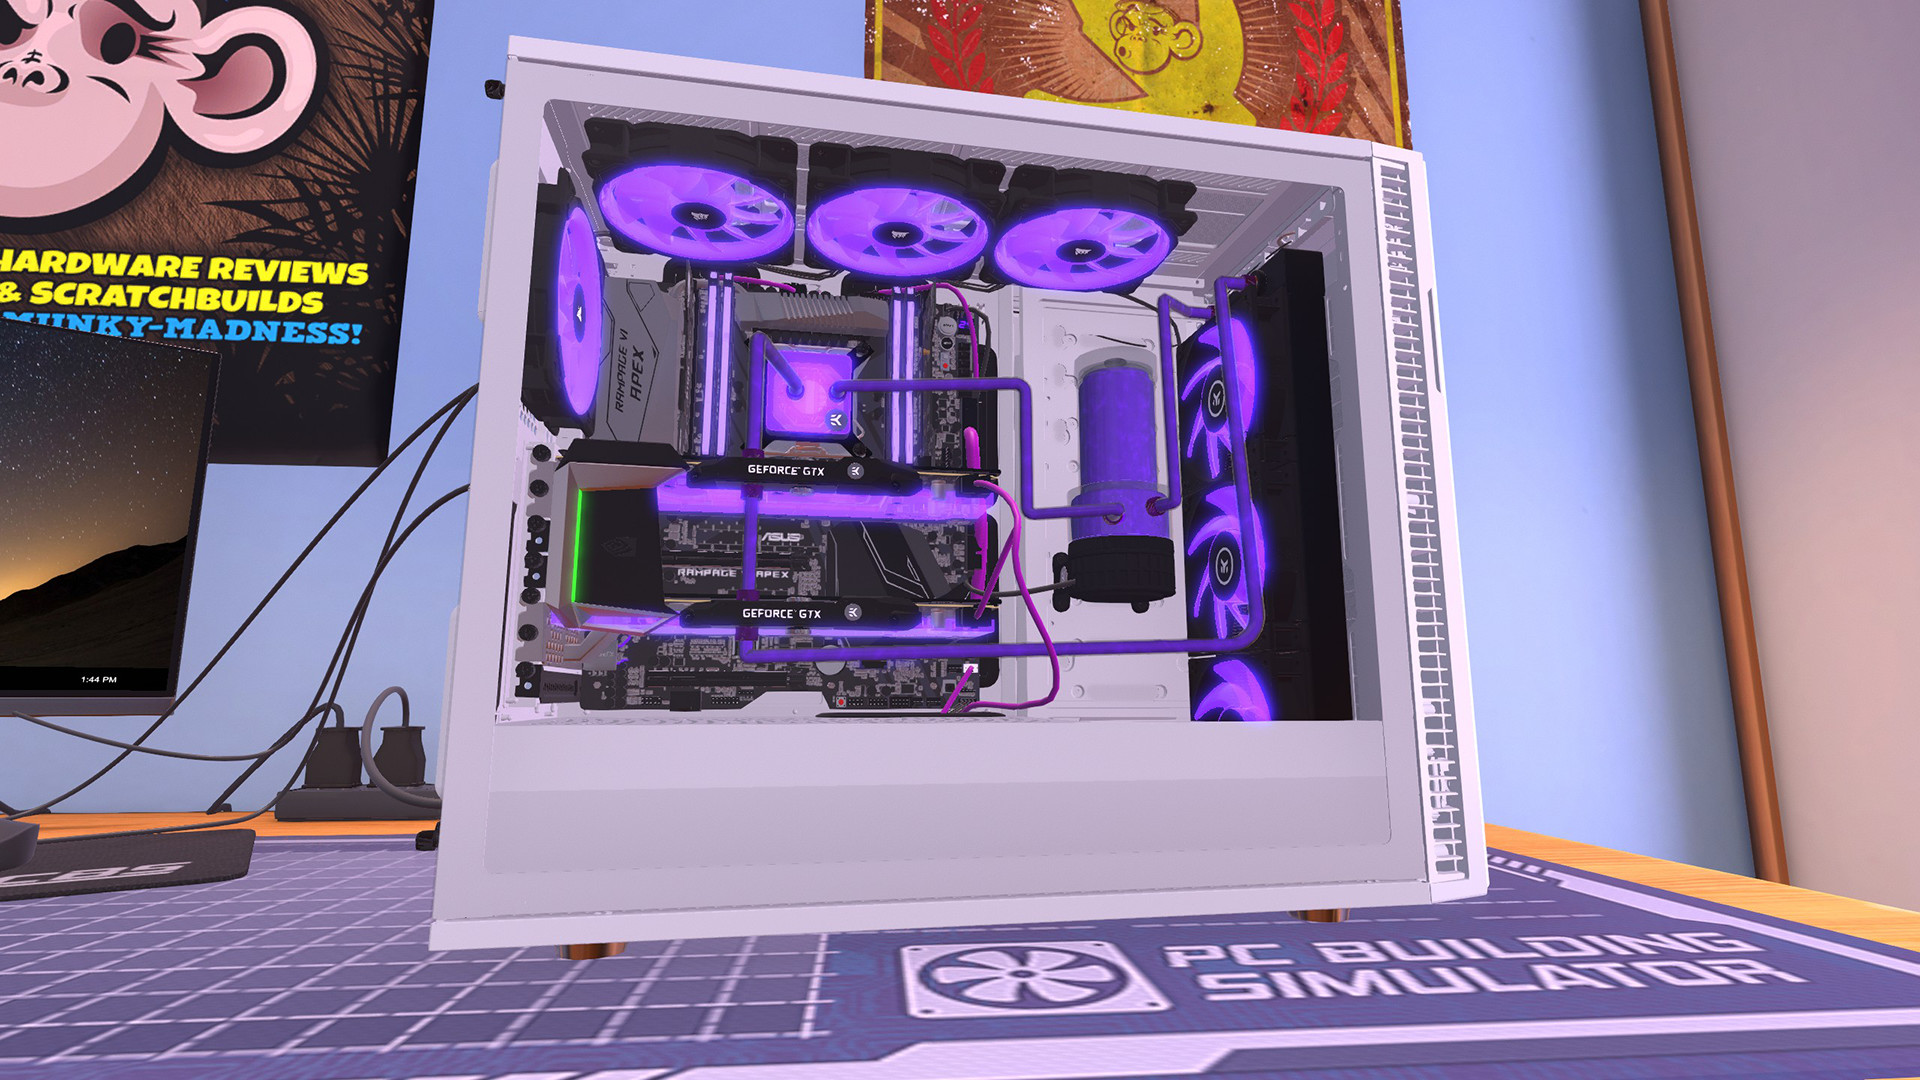
\includegraphics[width=0.45\textwidth]{Images/PCbuidlignSimulator1(2).jpg}
		\label{fig:pcbsbuild1}
	}%
	\hfil
	\subfigure[]{
		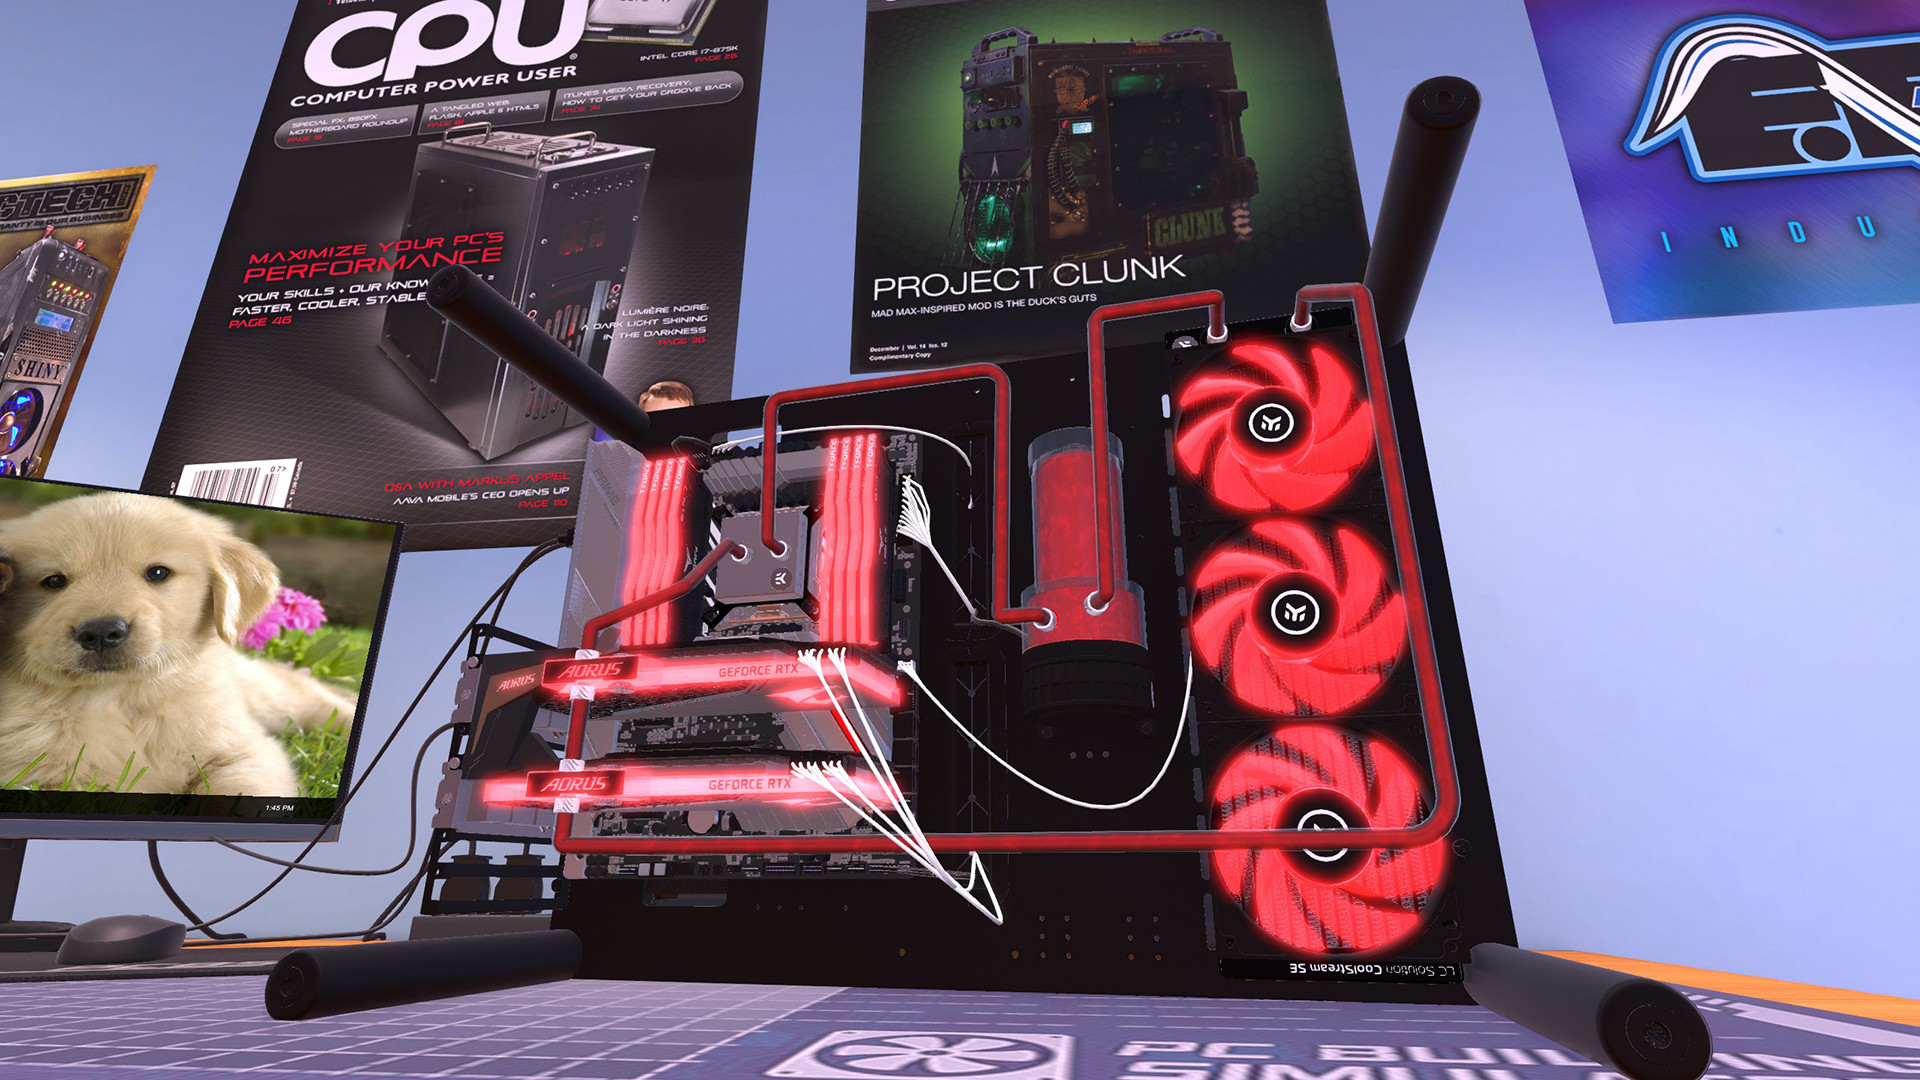
\includegraphics[width=0.45\textwidth]{Images/PCbuidlignSimulator1.jpg}
		\label{fig:pcbsbuild2}
	}
	\caption{Screenshots of a finished PCs made in PC Building Simulator from its Steam page}
\end{figure}

Figures \ref{fig:pcbsbuild1} and \ref{fig:pcbsbuild2} present possible PCs that can be built both in the game and in the real world, by utilizing mechanics and features described earlier.
Those possibilities are further expanded through the game's use of the Steam workshop feature, allowing players to make their own free DLCs.
This aspect of the game creates essentially endless options for assembling PCs that are realistic and feasible in the real world.

While PC Building Simulator is an incredibly comprehensive tool for gaining knowledge about PC building, it retains a rather low player count of an average of under 1000 unique players a month according to SteamDB.
Despite that, the game remains a popular and well-liked solution, as estimates of owned copies range from 1 to 4 million of both legally and illegally acquired copies.
Also, important factor in judging its usefulness is the reviews of its players on Steam.
Currently, there are slightly over 41 thousand reviews and 93\% of them are positive.

    \subsubsection{PC Building Simulator 2}

It is the second installment of the PC Building Simulator franchise, released on 12th October 2022.
It took the place of the best PC building simulator from its predecessor by implementing far more features and much better, more realistic graphics.
Also, its selection of components was vastly extended.

Just like the original PC Building Simulator, it has official partnerships with PC part manufacturers. However, this installment introduced many more than before, allowing for more niche parts to be included in an already large selection.
Also, unlike its predecessor, this game introduced partnerships with accessory producers like Thermal Grizzly, allowing for the players to get familiar with a wide selection of various PC building tools and products other than components like thermal pastes, pads, or even GPU stands.
Nonetheless, the biggest non-functional improvements upon the original are overhauled, realistic graphics; this is best showcased in Figure \ref{fig:pcbs2build}.

\begin{figure}[!ht]
	\centering
		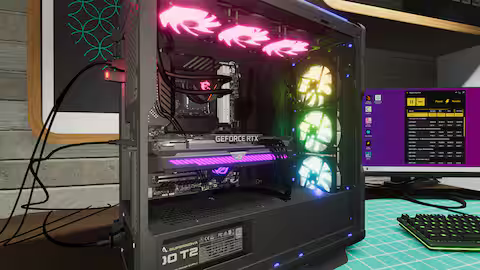
\includegraphics[width=0.65\textwidth]{Images/PCBuildingSim2.png}
	\caption{Screenshot of a finished PC made in PC Building Simulator 2 from Epic Games Store}
	\label{fig:pcbs2build}
    \end{figure}

The game also improved already revolutionary mechanics from the previous title by enhancing physics and models of all components.
This resulted in much better realism, but it also added many steps that were omitted in PC Building Simulator 1.
Some of the steps are:


\begin{itemize}
    \item Locking/unlocking CPU socket
    \item Application of thermal paste
    \item Installing I/O shields
\end{itemize}

While those steps tend to be mundane, they are crucial in building a functional PC and they require more precision than anyone expects.
Given that, PC Building Simulator 2 handles those and even more steps with a lot of care and realism.

Another new feature is the possibility to take apart some components like the GPU to further customize the PC by adding a less used water cooling block.
Also, it showcases how the GPU chipset actually looks like, giving players a far better understanding of what each component is.
Figure \ref{fig:pcbs2gpushipset} shows the taken apart GPU chipset being cleaned in-game, which is another new and interesting mechanic of this game.

\begin{figure}[!ht]
	\centering
		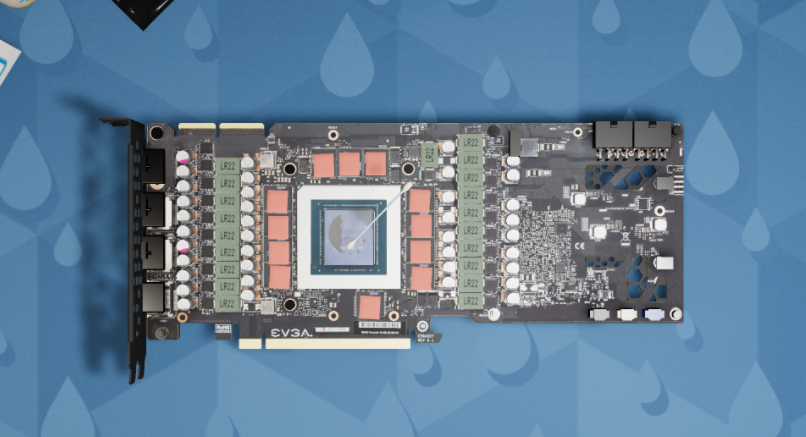
\includegraphics[width=0.7\textwidth]{Images/GPUChipsetPCBS2.png}
	\caption{Screenshot of a GPU chipset in PC Building Simulator 2 from Epic Games Store}
	\label{fig:pcbs2gpushipset}
    \end{figure}
    
Similarly to its predecessor, the game offers many tools to further customize virtual PCs.
Those tools consist of an expanded BIOS and even a fan curve control application; the latter is presented in figure \ref{fig:pcbs2fancurve}. 
Also, in this installment, the authors included benchmarks that simulate actual testing of assembled computers.

\begin{figure}[!ht]
	\centering
		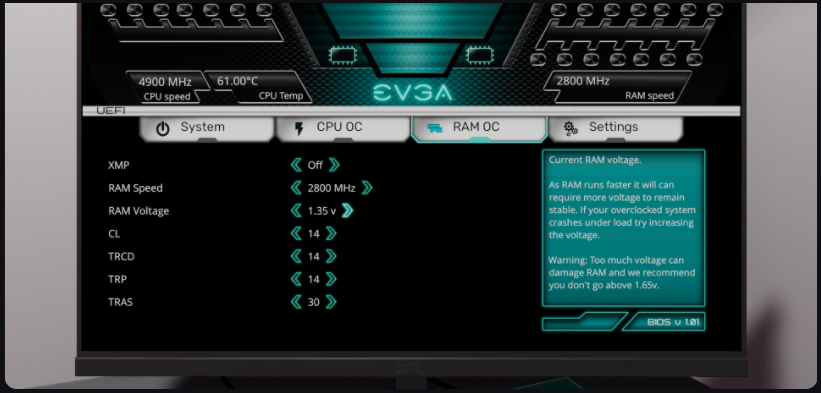
\includegraphics[width=0.7\textwidth]{Images/PCBS2FanCurveApp.png}
	\caption{Screenshot of fan curve application in PC Building Simulator 2 from Epic Games Store}
	\label{fig:pcbs2fancurve}
    \end{figure}

The aforementioned features already place it leagues above its predecessor and make it far better educational material on PC building.
However, the game has far more features that make it stand out.
With better graphics and physics, it reached a whole new level of visualization of the operation, and new customizing mechanics add new, less popular avenues to explore for those already advanced in PC assembly.

Unfortunately, this installment of the franchise didn't gather as much recognition as its predecessor.
Mainly, it is due to the choice of platform by the authors to sell their product, Epic Games Store.
It's worth mentioning that at the time of the game's release, Epic Games Store was widely hated for its exclusive program, which meant that any games under such contract could only be sold by Epic Games.
This combination led to an almost automatic decrease in the popularity of any games sold solely on this platform, and as we have discussed, PC Building Simulator 2 was one of the games that suffered from it.

\section{VR in hardware assembly and simulations}
\label{sec:VRGamesAndSimulations}

VR has seen increased use across a broad spectrum of industries, from gaming and education to medicine and engineering. In the context of hardware simulation, VR offers an immersive environment where users can interact with complex components and systems more intuitively. This makes it an increasingly promising tool for simulating physical tasks like PC building, especially for educational or training purposes.

\subsection{Advantages of using VR in hardware simulations}

Unlike traditional, more advanced simulations that use a regular 3D environment, simulations in VR offer much greater interactivity and immersion with users' surroundings.
Also, it allows for a simpler implementation solution as natural, even instinctive movements don't have to be coded, but only tracked.
This expands possible fields that can be simulated as  well as enhances angles from which working hardware can be observed, which adds another layer of precision.
In other words, using VR in hardware simulations provides the following benefits:

\begin{itemize}
    \item Immersive learning environment
    \item Safe space to experiment with hardware
    \item Real-time feedback on user interactions
    \item Fewer constraints on location or scene construction
\end{itemize}

\subsection{Existing VR hardware simulators}

As stated before, VR is an excellent environment for more advanced simulations.
And many game studios, university students, and researchers have taken that opportunity to fill the void.
Currently, there are countless VR simulators of many different kinds.
However, there aren't any about PC building; the closest we can find are those about assembling machines or robots.
That means that even though there are more simulators than one can count, VR still offers avenues to be explored.

\subsubsection{Virtual milling machine simulator}

This is an application made for Cave Automatic Virtual Environment (CAVE), focusing on the visualization of the operation of a specialized milling machine.
It was made in a specialized laboratory of Gdansk University of Technology by its students in 2020.

What makes this simulator stand out is the level of detail at which each component of the machine is simulated.
Each moving component is animated and in a CAVE environment, just like in VR, one can view the machine from different angles and notice things that simply are not possible in a traditional 3D setting on a monitor.
Such an approach allows for much better visualization of complex machines and opens new safe ways of understanding them.

Another interesting feature is the specialized graphical user interface (GUI), which is not made from a template like most do these days.
Rather, it uses field-specific icons and adds hints like names of parts the user points towards, which allows for a far smoother interaction with the simulated environment and understanding of how the simulated machine operates.

\subsubsection{Virtual Industrial Robot Assembly Simulator}

This is another application made for CAVE, however this one focuses on assembling an industrial robot from given parts.
It was made in a specialized laboratory of Gdansk University of Technology by HHN in 2019.

This application was developed as a trainer for building robots in a timely manner by following visual hints.
What makes this application interesting is that parts that the user is supposed to use to assemble his robot are placed on shelves around, which gives him a slight sense of challenge to match the visual hint to the part he/she has to use next.

The building mechanic is rather simple, the user has to grab the right part and drop it in close proximity to the visual hint.
The biggest challenge is to find the exact part, as all parts are placed on shelves around the player, and some of them are very similar to each other.
However, the scene makes it easier to quickly navigate between shelves and locate appropriate parts in a timely manner.
Nonetheless, the simulator shines with its intuitive controls and simple mechanics.

This simulator is a prime example of what VR hardware building simulations are like.
Most of them feature a simple grab and drop model, which at the same time is simple to implement and intuitive.
However, this particular application implemented a part recognition function, so that the user cannot place a part in the wrong order or place.

%\section{Interest in PC building}
%\label{sec:InterestInPCBuilding}

\chapter{TECHNOLOGIES AND TOOLS}
\label{chap:TechnologiesAndTools}

\section{Game engines}
\label{sec:GameEngines}

\section{Movement tracking devices}
\label{sec:MovementTrackingDevices}

\section{Programming environments}
\label{sec:ProgrammingEnviroments}

\chapter{SYSTEM PROJECT (Hubert Leszczyński)}
\label{chap:project}

The objective of the system is to create a trainer for assembling a personal computer, which can also visualize the computer's work.
The following chapter describes the project's functional and non-functional requirements, the necessary models and decisions which were the foundation for all of the implenentation processes.

\section{Project team}

The project team consists of four students from Gdańsk University of Technology.
Table \ref{tab:team} presents the team's skills and competencies.

\begin{table}[!ht]
\caption{Project team's competencies}
\label{tab:team}
\small
\begin{tabular}{|p{0.47\textwidth}|p{0.47\textwidth}|}
\hline
    %-
   \begin{center}
       \textbf{Name and surname}
   \end{center}  
   &
   \begin{center}
       \textbf{Skills}
   \end{center}
   \\\hline
   %-
    Jakub Jędrzejczyk 
    & \begin{itemize}
        \item Version Control
        \item Project infrastructure
        \item Leadership
        \item C++ and Java programming languages
        \item Interface design
        \item Computer games development
    \end{itemize} 
    \\\hline
    %-
    Hubert Leszczyński
    & \begin{itemize}
        \item C++ programming language
        \item Computer games development
        \item 3D graphics
        \item Project modeling
    \end{itemize}
    \\\hline
     %-
    Jakub Kinder
    & \begin{itemize}
        \item Creating computer games
        \item UE 5
        \item C++ and C\# programming languages
    \end{itemize}
    \\\hline
     %-
    Mateusz Merda
    & \begin{itemize}
        \item Creating computer games
        \item Programming
        \item Sound management
        \item Creating UI
    \end{itemize}
    \\\hline
    %-
\end{tabular}
\end{table}
\section{Project timetable}

Table \ref{tab:timetable} presents project's team timetable and objectives for each month.

\begin{table}[H]
\caption{Project team's timetable}
\label{tab:timetable}
\small
\begin{tabular}{|p{0.47\textwidth}|p{0.47\textwidth}|}
\hline
    %-
   \begin{center}
       \textbf{Month 2025}
   \end{center}  
   &
   \begin{center}
       \textbf{Objective}
   \end{center}
   \\\hline
    %-
    March
    &
    Team introduction to the CAVE system and its applications
    \\\hline
   %-
    April 
    &
    Functional and non-functional requirements specification
    \\\hline
    %-
    April-May
    & Review of the literature
    \\\hline
    %-
    May
    & System project and modeling
    \\\hline
     %-
    June
    & Creation and configuration of the project repository
    \\\hline
     %-
    June
    & Implementation of trainee's movement logic
    \\\hline
     %-
    September
    & Creating 3D models
    \\\hline
     %-
    September
    & Implementation of computer components manipulation
    \\\hline
     %-
    October
    & Implementation of computer assembly logic
    \\\hline
    %-
    October
    & 3D models validation
    \\\hline
     %-
    October-November
    & Integration of the application with the VR CAVE
    \\\hline
     %-
    November
    & Testing of the application's progress in CAVE
    \\\hline
    %-
    November
    & Implementation of the component state visualization
    \\\hline
     %-
    November-December
    & Conducting application's tests on a group of users
    \\\hline
     %-
    December
    & Implementation of trainee's score calculation and trainee support
    \\\hline
    %-
    December
    & Final tests on CAVE
    \\\hline
    %-
    December
    & Completion of the project's documentation
    \\\hline
    %-
\end{tabular}
\end{table}
% popraw
\section{Project assumptions}
During the work on the system project the team was able to establish the assumptions for the final vision of the application.
The work on the project must be limited by the following assumptions and the application must comply with all of its requirements.
\subsubsection{Project characteristics}
The target application must be developed as a 3D system developed using the UE 5 game engine.
The system's architecture must follow a hybrid approach, where the logic of the application is implemented using both C++ programming language and UE5 Blueprints scripts.
The application requires a basic UI created using computer graphics.
The system is intented to be used by a single trainee.
\subsubsection{Project work environment}
The project application must operate in the CAVE system of Gdańsk University of Technology, which consists of two disctinct CAVEs:
\begin{itemize}
    \item Small CAVE - a setup of four monitors equiped with a head movement tracker and two hand controllers,
    \item Large CAVE - a cube composed of six screens, each with the side length of 3,4 meters, equipped with two tracking sensors on each side.
\end{itemize}
The synchronization between the screens and tracking sensors must be achieved using freely available UE 5 assets.
\subsubsection{Constraints}
Due to the application's architecture, it will not be working on PCs and mobile devices.

\subsection{Functional requirements}
The functional requirements describe the actions that the system must perform to work correctly.
Each functional requirement has to be thoroughly specified, analyzed, and assigned with an appropriate priority.
The priorities in this project were determined using the  MoSCoW (Must, Should, Could, Won't) scale.
Table \ref{tab:functionalRequirements} presents the functional requirements of the target application.
\begin{table}[!ht]
\caption{Functional requirements}
\label{tab:functionalRequirements}

\small
\begin{tabular}{|p{0.38\textwidth}|p{0.38\textwidth}|p{0.18\textwidth}|}
\hline

    %-
   \begin{center}
       \textbf{Requirement}
   \end{center}  
   &
   \begin{center}
       \textbf{Description}
   \end{center}
   &
   \begin{center}
       \textbf{Priority}
   \end{center}
   \\\hline
   %-
    Trainee's movement detection
    & Trainee's movement has to be detected by the CAVE system, and their position must be updated in the application.
    & Must
    \\\hline
     %-
    Computer component manipulation
    & The trainee must be able to fully manipulate the computer components by moving them and installing them into the compatible slots.
    & Must
     \\\hline %-
    Tracking the progress of virtual computer assembly
    & The application must inform the trainee about the progress of the virtual computer assembly and detect the completion of this process.
    & Must
    \\\hline %- 
    Components state visualization
    & The application should allow to visualize the state of the computer components in a fully assembled virtual computer.
    & Should
    \\\hline %-
    Assembly grading
    & The trainee's score can be calculated using several factors, such as assembly speed or a number of their mistakes.
    & Could
    \\\hline %-
    Trainee support
    & The computer component slots can be highlighted to guide the trainee in the virtual computer assembly process.
    & Could
    \\\hline
\end{tabular}
\end{table}

\subsection{Non-functional reuirements}

Non-functional requirements are the factors that determine the quality attributes of a software system, such as its portability, performance or maintainability.
Rather than defining how the system works, they describe how it performs under specific conditions.
These requirements play an important role during software development, as they serve as criteria for selecting different designs and approaches \cite{NonFunctionalRequirements}.
Table \ref{tab:nonFunctionalRequirements} presents the trainer's non-functional requirements.

\begin{table}[!ht]
\caption{Non-functional requirements}
\label{tab:nonFunctionalRequirements}

\small
\begin{tabular}{|p{0.38\textwidth}|p{0.38\textwidth}|}
\hline

    %-
    \begin{center}
       \textbf{Requirement category}
    \end{center}  
    &
    \begin{center}
        \textbf{Description}
    \end{center}
    \\\hline
    %-
    Performance
    & The trainer must support multiple screens without visual artifacts. The application should also provide the trainee with a smooth frame rate above 60 frames per second.
    \\\hline
    %-
    Responsiveness
    & A latency between the trainee's actions and an application's reaction must not exceed 20 ms.
    \\\hline
    %-
    Reliability
    & The application must behave correctly for a single trainee.
    \\\hline
    %-
    Usability
    & The application's interface should be intuitive and easy to use for the trainee.
    \\\hline
    %-
    Maintainability
    & The application's code and resources should be easy to maintain by the developers.
    \\\hline
    %-
    Extensibility
    & The application should allow developers to easily add new functionalities and objects.
    \\\hline
\end{tabular}
\end{table}

\section{Use cases}
A use case is a singular unit of system functionality, which can be described as a sequence of interactions between the system and its users.
Use cases have wide application in software engineering and system design, allowing for extensive planning of system requirements before implementing any functionality.
The most popular way to use them is to model the UML (Unified Modeling Language) diagram.
This type of diagram can identify all the system use cases, their dependencies, and also the user groups.
In our project, we have decided to divide the diagram into two parts.
\subsection{Trainee movement use cases}
Figure \ref{fig:movementDiagram} illustrates the first use case diagram of the two, which describes the use cases for detecting the movement of the trainee and its dependence on the components of the trainer. 
Each use case requires the VR CAVE sensors to work.
\begin{figure}[H]
	\centering
		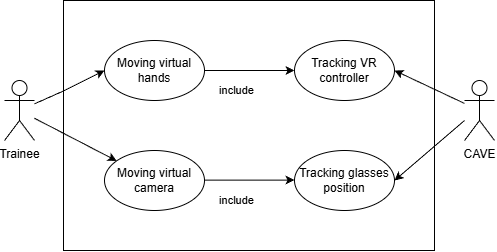
\includegraphics[width=0.7\textwidth]{Images/TraineeMovementUseCases.png}
	\caption{Use case diagram for trainee movement}
	\label{fig:movementDiagram}
\end{figure}
The use case descriptions for controlling trainee's movement are detailed in following subsections.

\subsubsection{Detecting trainee's position}
\begin{itemize}
\item Actors: Trainee, CAVE Sensors
\item Description: The system detects the change of the trainee's position.
\item Prerequisites: None.
\item Post-requisites: Data of the trainee's position is forwarded to the application's components.
\item Scenario: 
\begin{enumerate}
    \item The trainee moves inside CAVE.
    \item CAVE sensors read the trainee's movement data based on the VR controllers and glasses positions.
    \item The updated data is forwarded to the application's components.
\end{enumerate}

\end{itemize}
\subsubsection{Tracking VR controllers}
\begin{itemize}
\item Actors: Trainee, CAVE Sensors
\item Description: The system detects the change of the position or rotation of the VR controller.
\item Prerequisites: None.
\item Post-requisites: Data of the trainee's hand movement is forwarded to the application's components.
\item Scenario: 
\begin{enumerate}
    \item The trainee moves or rotates their hand.
    \item CAVE sensors read the updated position of VR controllers.
    \item The updated data is forwarded to the application's components.
\end{enumerate}
\end{itemize}

\subsubsection{Virtual hands movement}

\begin{itemize}
\item Actors: Trainee
\item Description: Virtual hands' position and rotation are updated according to trainee's movement.
\item Prerequisites: VR controllers movement or the trainee's position change were detected (Use cases: Detecting trainee's position, Tracking VR controllers).
\item Post-requisites: Virtual hands position parameters are updated.
\item Scenario: 
\begin{enumerate}
    \item The updated position and rotation vectors are read from the player control component.
    \item Virtual hands' position and rotation vectors are updated with the read values. 
\end{enumerate}

\end{itemize}

\subsection{Computer assembly use cases}
Figure \ref{fig:assemblyDiagram} illustrates the second use case diagram, describing the use cases for the computer assembly process, along with mechanics of trainee's score calculation and the computer work visualization.
\begin{figure}[H]
	\centering
		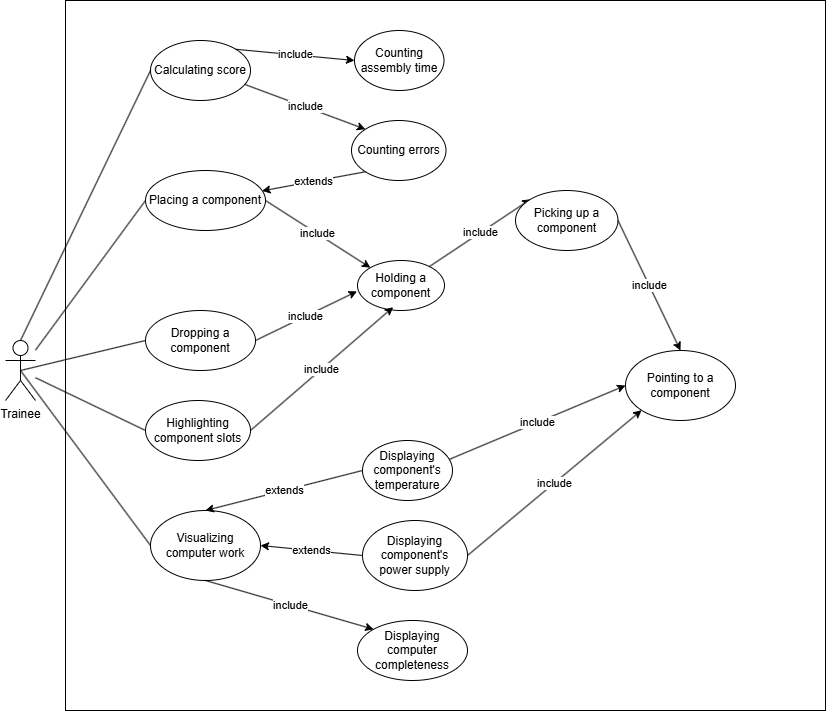
\includegraphics[width=0.7\textwidth]{Images/AssemblyUseCases.png}
	\caption{Use case diagram for computer assembly}
	\label{fig:assemblyDiagram}
\end{figure}

\noindent The following subsections provide the descriptions for the use cases.
\subsubsection{Detecting a holdable object}
\begin{itemize}
\item Actors: Trainee
\item Description: System detects the overlaps between a virtual hand and holdable objects.
\item Prerequisites: Virtual hand object is overlapping with one or more holdable objects.
\item Post-requisites: A holdable object becomes highlighted.
\item Scenario: 
\begin{enumerate}
    \item Trainee moves the virtual hand towards a holdable object.
    \item The system detects an overlap between a virtual hand and another object.
    \item A holdable object becomes highlighted using the virtual hand's color.
\end{enumerate}
\item Alternate scenario: The virtual hand object overlaps with multiple holdable objects at once.
\begin{enumerate}
    \item The system compares all of the objects overlapping with a virtual hand.
    \item The object with the smallest volume becomes selected and highlighted.
\end{enumerate}
\end{itemize}

\subsubsection{Picking up an object}
\begin{itemize}
\item Actors: Trainee
\item Description: Trainee picks up a holdable object.
\item Prerequisites: Holdable object overlaps with a virtual hand (Use case: Detecting a holdable object).
\item Post-requisites: A holdable object follows trainee's hand.
\item Scenario: 
\begin{enumerate}
    \item Trainee presses a trigger on the controller.
    \item System detects trainee's action.
    \item A holdable object begins following trainee's hand.
\end{enumerate}

\end{itemize}
\subsubsection{Holding an object}
\begin{itemize}
\item Actors: Trainee
\item Description: A held object's position and rotation follow the virtual hand.
\item Prerequisites: Trainee picks up a holdable object (Use case: Picking up an object).
\item Post-requisites: The held object continuously follows the virtual hand and updates its position and rotation.
\item Scenario: 
\begin{enumerate}
    \item The held object reads virtual hand object's position and rotation.
    \item The held object's position and rotation are updated with the obtained values.
\end{enumerate}
\end{itemize}

\subsubsection{Releasing an object}
\begin{itemize}
\item Actors: Trainee
\item Description: A holdable object becomes released and stops following trainee's virtual hand.
\item Prerequisites: Trainee holds an object (Use case: Holding an object).
\item Post-requisites: A held object either falls to the ground or becomes installed in the virtual computer (Use case: Installing a computer component).
\item Scenario: 
\begin{enumerate}
    \item Trainee presses a trigger on the controller.
    \item The released object stops being highlighted.
    \item The held object stops following trainee's hand.
    \item The released object falls to the ground.
\end{enumerate}
\item Alternate scenario: The released object is a computer component.
\begin{enumerate}
    \item The system checks whether the male slot of the released component overlaps with a female slot of another component.
    \item If the condition is met, the system attempts to install the released component in the slot it's overlapping with (Use case: Installing a computer component).
    \item Otherwise, the released component falls to the ground.
\end{enumerate}
\end{itemize}

\subsubsection{Installing a computer component}
\begin{itemize}
\item Actors: Trainee
\item Description: A computer component becomes intalled in the matching slot.
\item Prerequisites: Trainee releases the computer component while it overlaps with a component slot (Use case: Releasing an object).
\item Post-requisites: The computer component is either installed in the component slot or it falls to the ground.
\item Scenario: 
\begin{enumerate}
    \item Trainee releases the held object.
    \item System checks whether the component type matches the type of the slot it overlaps with.
    \item If the types match, the computer component's position becomes fixed and it snaps to the slot.
\end{enumerate}
\item Alternate scenario: The component is not compatible with the slot.
\begin{enumerate}
\item The released computer component falls to the ground.
\item The error counter increments (Use case: Counting trainee's errors).
\end{enumerate}
\end{itemize}


\subsubsection{Removing the computer component}
\begin{itemize}
\item Actors: Trainee
\item Decription: A computer component is removed from the slot.
\item Prerequisites: A computer component selected for removal is installed into one of the slots.
\item Post-requisites: Removed computer component falls down and can be picked up again.
\begin{enumerate}
    \item Trainee's virtual hand overlaps with an installed component (Use case: Detecting a holdable object).
    \item Trainee presses the button on a controller.
    \item System detects trainee's action.
    \item Removed component stops following the slot it was removed from.
\end{enumerate}


\end{itemize}

\subsubsection{Visualizing component's state}
\begin{itemize}
\item Actors: Trainee
\item Description: The parameters of a computer component is displayed to the trainee.
\item Prerequisites: Computer is fully built.
\item Post-requisites: Trainee sees component's state.
\item Scenario: 
\begin{enumerate}
    \item The trainee's virtual hand overlaps with a computer component installed in the virtual computer (Use case: Detecting a holdable object).
    \item System reads component's data.
    \item Read data is displayed to the trainee using an application's interface.
\end{enumerate}

\end{itemize}

\subsubsection{Displaying assembly progress}
\begin{itemize}
\item Actors: Trainee
\item Description: The system informs the trainee about the progress of the virtual computer assembly as a list of objectives.
\item Prerequisites: The trainee installs a computer component (Use case: Installing a computer component).
\item Post-requisites: The system updates and displays the list of objectives according to the virtual computer assembly progress.
\item Scenario: 
\begin{enumerate}
    \item The system checks which components are installed in the virtual computer.
    \item The system updates the list of objectives accordingly to the progress of the virtual computer assembly.
    \item The system displays the updated list of objectives in an application's interface.
\end{enumerate}
\end{itemize}

\subsubsection{Visualizing computer work}
\begin{itemize}
\item Actors: Trainee
\item Description: The system displays information about the virtual computer assembly progress or a state of the computer components to the trainee.
\item Prerequisites: None.
\item Post-requisites: The system presents necessary information using an application's interface.
\item Scenario: 
\begin{enumerate}
    \item The system validates the state of the virtual computer.
    \item If the virtual computer is not fully assembled, the system displays information about the progress of the assembly process (Use case: Displaying assembly progress).
\end{enumerate}
Alternate scenario: The virtual computer is fully assembled and the virtual hand object is overlapping with one of its components (Use case: Detecting a holdable object).
\begin{enumerate}
    \item The system displays information about the component's state to the trainee (Use case: Visualizing component's state).
\end{enumerate}
\end{itemize}


\subsubsection{Counting assembly time}  
\begin{itemize}
\item Actors: Trainee
\item Description: Time of the assembly is presented to the trainee.
\item Prerequisites: Trainee picks up a computer component for the first time (Use case: Picking up an object).
\item Post-requisites: Time becomes displayed in the application's interface.
\item Scenario: 
\begin{enumerate}
    \item System checks if the computer assembly process is not finished.
    \item System calculates the elapsed assembly time.
    \item The time value becomes displayed in the application's interface clock object.
\end{enumerate}
Alternate scenario: The computer assembly is finished.
\begin{enumerate}
    \item The clock object stops updating the time.
\end{enumerate}
\end{itemize}

\subsubsection{Counting trainee's errors}
\begin{itemize}
\item Actors: Trainee
\item Description: The system counts the trainee's mistakes during the virtual computer assembly process.
\item Prerequisites: Trainee installs a computer component in an incompatible slot (Use case: Installing a computer component). 
\item Post-requisites: Error counter is updated and displayed in the application's interface.
\item Scenario: 
\begin{enumerate}
    \item System increments the error counter.
    \item The updated error count becomes displayed in the application's interface.
\end{enumerate}

\end{itemize}

\subsubsection{Tracking trainee's score}
\begin{itemize}
\item Actors: Trainee
\item Description: Trainee's score is calculated based on the time and quality of a computer assembly process.
\item Prerequisites: The virtual computer is fully assembled.
\item Post-requisites: The trainee's score is displayed in an application's interface.
\item Scenario: 
\begin{enumerate}
    \item The trainee's score is initialized with a constant value.
    \item The system decreases the score by a constant value for each 10 seconds of the assembly process (Use case: Counting assembly time).
    \item The system decreases the score by a constant value for each mistake made by the trainee (Use case: Counting trainee's errors).
    \item System displays score in the application's interface.
\end{enumerate}

\end{itemize}
% popraw
\section{Classes}
\label{sec:classes}
A class is a fundamental element of OOP (Object-Oriented Programming).
It's a definition describing an object's state or behaviour using certain attributes or methods. 
The following subsections presents the developed classes along with the class diagram.
\subsection{Class diagram}
A class diagram is an essential element of a system project.
It allows to visualize the project's structure as well as relationships and dependencies of the classes.
Figure \ref{fig:movementDiagram} provides a full class diagram for the project.
\begin{figure}[H]
	\centering
		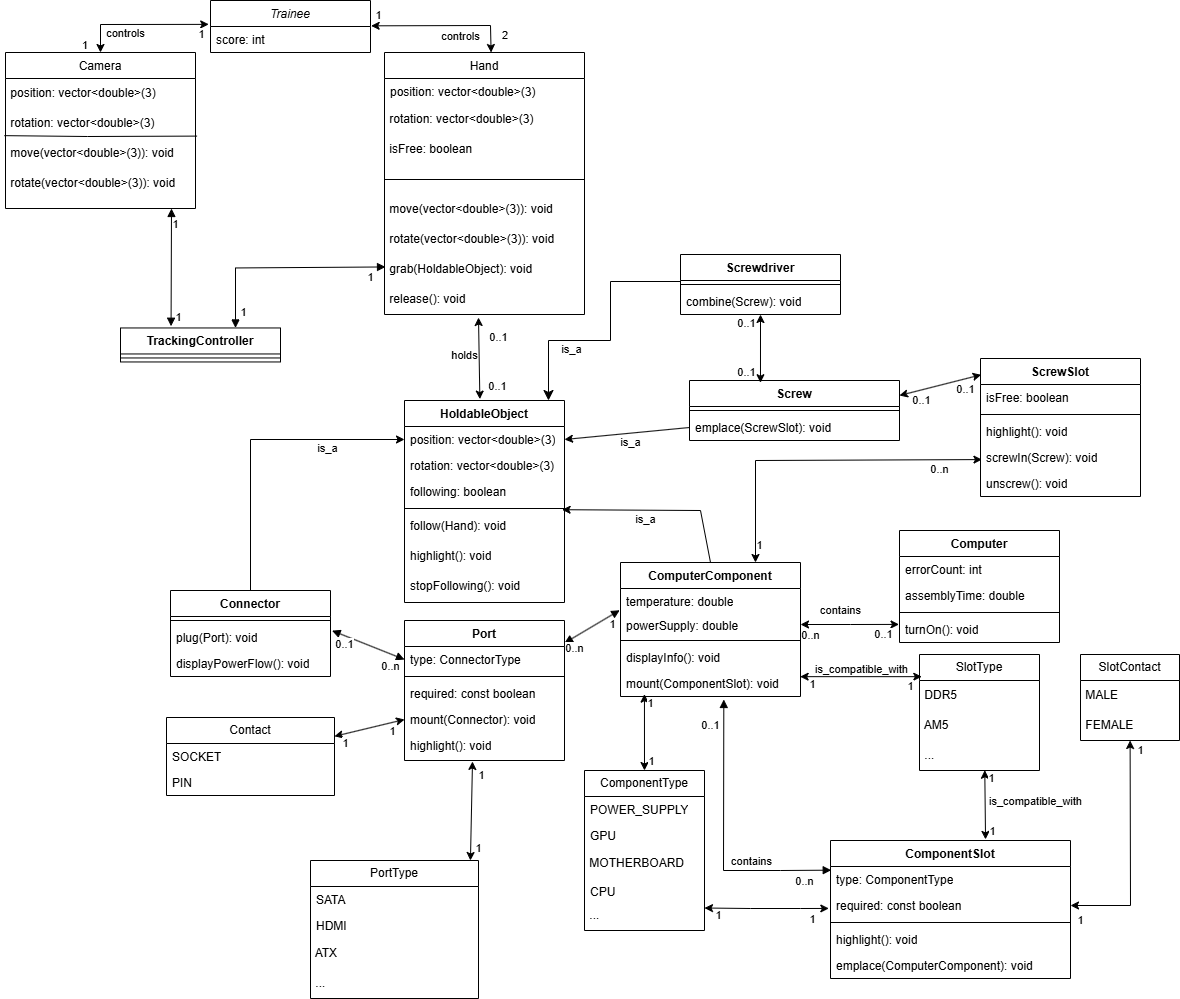
\includegraphics[width=0.7\textwidth]{Images/Class_diagram.png}
	\caption{Class diagram}
	\label{fig:ClassDiagram}
\end{figure}
The trainee-related classes (figure \ref{fig:TraineeClasses}) are responsible of detecting trainee's movement and calculating their score.
A Camera class describes the behavior of a virtual camera object, which acts as a trainee's point of view in a VR environment.
The Hand class is responsible for moving the virtual hands objects.
Both of the described classes are using the TrackingController class, which is responsible for detecting the movement of a trainee in the VR CAVE and forwarding its data to these classes.
\begin{figure}[H]
	\centering
		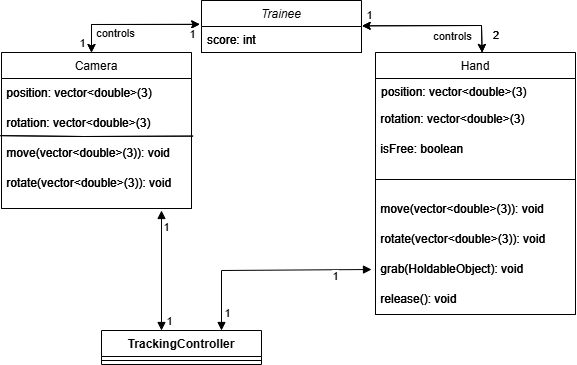
\includegraphics[width=0.7\textwidth]{Images/TraineeRelatedClasses.png}
	\caption{Trainee-related classes}
	\label{fig:TraineeClasses}
\end{figure}
A HoldableComponent class (figure \ref{fig:HoldableComponentClasses}) describes each object, which can be manipulated by trainee by holding it and moving it around.
These classes are elements or tools required to build a virtual computer.
If the trainee grabs one of these objects and moves, the held object should follow their hands' position.
Releasing the held object makes it fall to the ground and return to its initial position.

\begin{figure}[H]
	\centering
		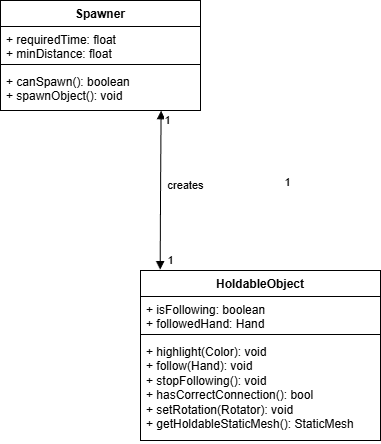
\includegraphics[width=0.7\textwidth]{Images/HoldableComponentClasses.png}
	\caption{Holdable Components classes}
	\label{fig:HoldableComponentClasses}
\end{figure}

A Connector class (figure \ref{fig:ConnectorRelatedClasses}) describes objects, which connect two or more computer components with eahc other.
Each connector has one or more ports.
Every port is described by a type and a contact, which are stored in PortType and Contact enumeration classes.
To properly mount a connector, all of his ports have to be connected with a port of the same type and an opposite contact. 
The power flow of the connectors may also be visualized after turning on a fully built computer. 
\begin{figure}[H]
	\centering
		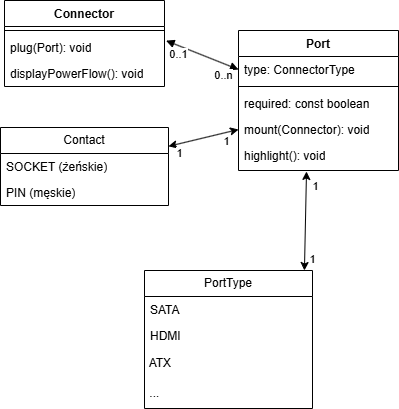
\includegraphics[width=0.7\textwidth]{Images/ConnectorRelatedClasses.png}
	\caption{Connector-related classes}
	\label{fig:ConnectorRelatedClasses}
\end{figure}
Figure \ref{fig:ToolsRelatedClasses} presents the Screwdriver and Screw classes, which describe the objects for tools used during the virtual computer assembly.
A held screwdriver object can be connected with a screw by contacting them with each other.
A screw can be emplaced in a ScrewSlot object, when a trainee holds the connected screwdriver and screw objects, moves their hand near the slot and rotates it.

\begin{figure}[H]
	\centering
		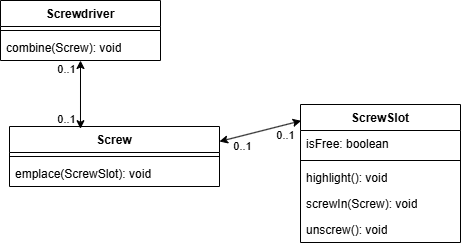
\includegraphics[width=0.7\textwidth]{Images/ToolsRelatedClasses.png}
	\caption{Tools-related classes}
	\label{fig:ToolsRelatedClasses}
\end{figure}


A virtual computer (figure \ref{fig:ComputerRelatedClasses}) consists of multiple computer components.
Each computer component object can be mounted in a ComponentSlot object.
To mount a component in a slot, the types of the component and the slot, which are listed in ComponentType and PortType enumerations, must be equal.
Some components may contain connector ports and slots for the screws or another components.
Most of the components have parameters which values may be continously changing and visualized after turning on a fully built computer.

\begin{figure}[H]
	\centering
		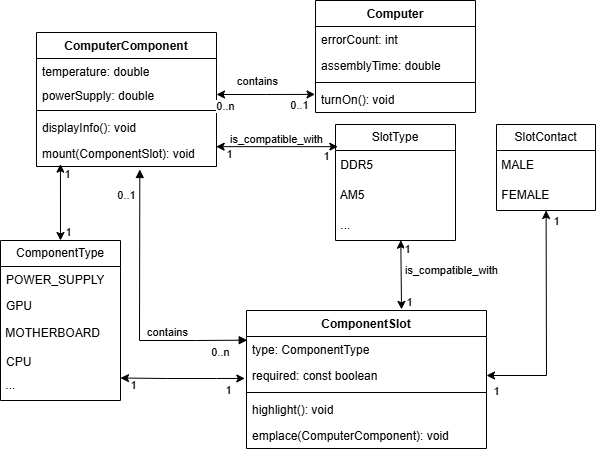
\includegraphics[width=0.7\textwidth]{Images/ComputerRelatedClasses.png}
	\caption{Computer-related classes}
	\label{fig:ComputerRelatedClasses}
\end{figure}
\chapter{IMPLEMENTATION, TESTING AND VALIDATION}
\label{chap:implementation}

\subsection{System implementation}

\subsection{System testing}

\subsection{System evaluation}

\chapter{SUMMARY} 
This chapter presents results of the project, descriptions of its current state, achieved goals, our conclusions and future plans.

\section{Results (Jakub Kinder)}
\label{sec:results}
Through the course of this diploma project, we managed to complete most of our goals, notably we created a functional and visually pleasing PC building trainer for CAVE.
It possesses the desired core functionalities and is made in a fashion that allows it to be scalable which is important for future improvements.

In its current state, the developed application allows players to properly interact with provided PC components using Hand mechanics presented in \autoref{chap:ObjectHolding}.
Also, it possesses correct component connection mechanic described in \autoref{chap:ConnectingComponents} as well as progress tracking system, \autoref{chap:buildmanager}.
Furthermore, the trainer boasts helpful GUI elements in form of the clock measuring building time, task list, which guides novice PC builders through most common PC building procedure as well as information panel for each PC part, described in depth in \autoref{chap:GUI}.
The application, also features cables, that are essential part of PC building, however, due to their late appearance in the project they still need refinement.



\section{Conclusions}

\section{Future plans (Jakub Jędrzejczyk)}
\label{sec:FuturePlans}

\subsection{Bugfixes (Jakub Jędrzejczyk)}

Despite our best efforts to test the code before finalizing the release for user testing purposes, a few bugs have been identified that ought to be addressed, should work continue on this project.

The most glaring issue is the fact that the AMD CPU compatible motherboard's RAM slots fail to connect to any of the available RAM modules.
This is likely caused by misconfiguration of either of the problematic components' slot definitions, and should be relatively straightforward to fix.
% to się poprawi szybko i zmieni na czas przeszły

Another issue is that sometimes if a slot overlaps two slots (one valid, one invalid to place the part in), the connected component might end up attached to the invalid slot instead of the valid one, if the user decides to make the connection.
During testing, users were instructed to do their best to ensure a component's slot only overlapped a single, valid slot, but we recognize that this is not a viable, long-term solution.
This issue may stem from unexpected behavior in the event binding algorithm, and will require further investigation.
% tutaj pewnie obrazk z porównaniem dobrego i złego zachowania

While connections between components work as intended, there is a very rare bug in which the component being connected may end up moving not towards the slot it is being connected to, but rather towards the very centre of the target component (i.e. the parent of the target slot).
Given how otherwise reliable this functionality is, this may again be an issue in the event binding, as it appears as though the would-be parent is instead treated as the released component, making it the child of the connection.
% przykład, dobry byłby procesor który się połączył do środka płyty głównej zamiast do slotu

These are all the bugs that have been identified so far.
Whereas the first was easy to fix and has already been addressed, the other two will require further investigation and testing to ensure they are properly resolved.
Fortunately, none of these bugs make it impossible to use the application, though in the context of an otherwise polised product, they do detract from the overall user experience.
As known and documented issues, these would be the first to be addressed, should further development of the project be undertaken.

\subsection{Controller Joystick Rotation Fixes (Jakub Jędrzejczyk)}
\label{sec:ControllerJoystickRotationFixes}

The most raised issue by testers (as per subchapter \ref{sec:user-testing-results}) was the difficulty in rotating components using the joystick on the VR controllers.
While the development team found the rotation mechanics to be a helpful part of the building process, the users found it unintuitive and cumbersome, often leading to frustration and mistakes, requiring a lot of trial and error to get the desired orientation of components.
We believe this to be caused by the fact that most users chose this method of rotation over physically rotating their hands, and while a more in-depth tutorial on how to use the joystick rotation could help alleviate this issue, it may still be necessary to rework the rotation mechanics entirely.

The current implementation uses rotation axes fixed to the objects, which mean that a held object's rotation changes relative to its current orientation.
This means that if a user rotates an object 90 degrees on one axis, the other axes also change their orientation relative to the user, making further rotations possibly confusing.
A better approach would most likely be to use world space axes for rotation, meaning that no matter the current orientation of the object, pushing the joystick up would always rotate the object around the world's X axis, pushing it right would always rotate it around the world's Y axis.
Doing so would most likely require modification of the way a holdable object utilizes the RotatingMovement component, which by default uses local space axes for rotation.

Once done, this feature ought to be tested again with users to verify that the new rotation mechanics meet their expectations.

Additionally, it may be worth considering adding visual aids to help users understand the rotation mechanics better, particularly hinting about what direction the object should be rotated to fit into a slot.

\subsection{Data-driven components (Jakub Jędrzejczyk)}
\label{sec:DataDrivenComponents}

Originally, the available components were planned to be loaded dynamically using sets of files consisting of descriptions in JSON \cite{brayRFC8259JavaScript2017} format and model files.
The JSON files would contain all the necessary information about the object, such as its name, description, paths to the model files, specifications, component slots, their sizes, etc. 
The models would be in glTF 2.0 \cite{ISOIEC12113} format, which is a modern format for 3D models, supporting PBR materials and animations.

This approach allows for less coupling between the application and the content, and is an approach used in games such as Factorio, Sid Meier's Civilization, and, more recently, Minecraft (as many of the 2025 patches have focused on decoupling content from the core game engine).
% przydałyby się cytaty
This approach usually introduces higher up-front development time, as on top of the core functionality and content loading systems, tools for content creation and validation need to be developed.
The result, however, means that should development on the core application cease, users can freely extend the application's lifespan, even within the limits of existing functionality.

These plans were partially implemented, with a basic object loading system being created, but quickly deprioritized in favor of core functionality described previously.
Due to time constraints, the aforementioned tools for content creation and validation could not be created, with the current content being implemented entirely within Unreal Engine 5.

The planned functionality would require two blueprints - the first one would be responsible for scanning the folder with content in search of JSON files, while the second would spawn an object based on the description passed to it.
Each folder in the UserContent (made specifically for the purpose of allowing content to be edited by the User) directory would be treated as a category for objects to be sorted into (GPU, CPU, etc.).
% cytat potrzebny
Each one of these directories would then be read, and the object's description would be indexed within the application.
Given a wide selection of components, this would require relatively small memory footprint, with models and in-engine objects only being created on-demand, e.g. when a user selects a component from a list to be spawned in the scene.
The second blueprint would then load the model and create an appropriate object based on the description provided.

In the future, should this functionality be revisited, such a system could be implemented using serialization and deserialization techniques, allowing for usage of already implemented components as reference for future ones.

% \begin{figure}[H]
% 	\centering
% 		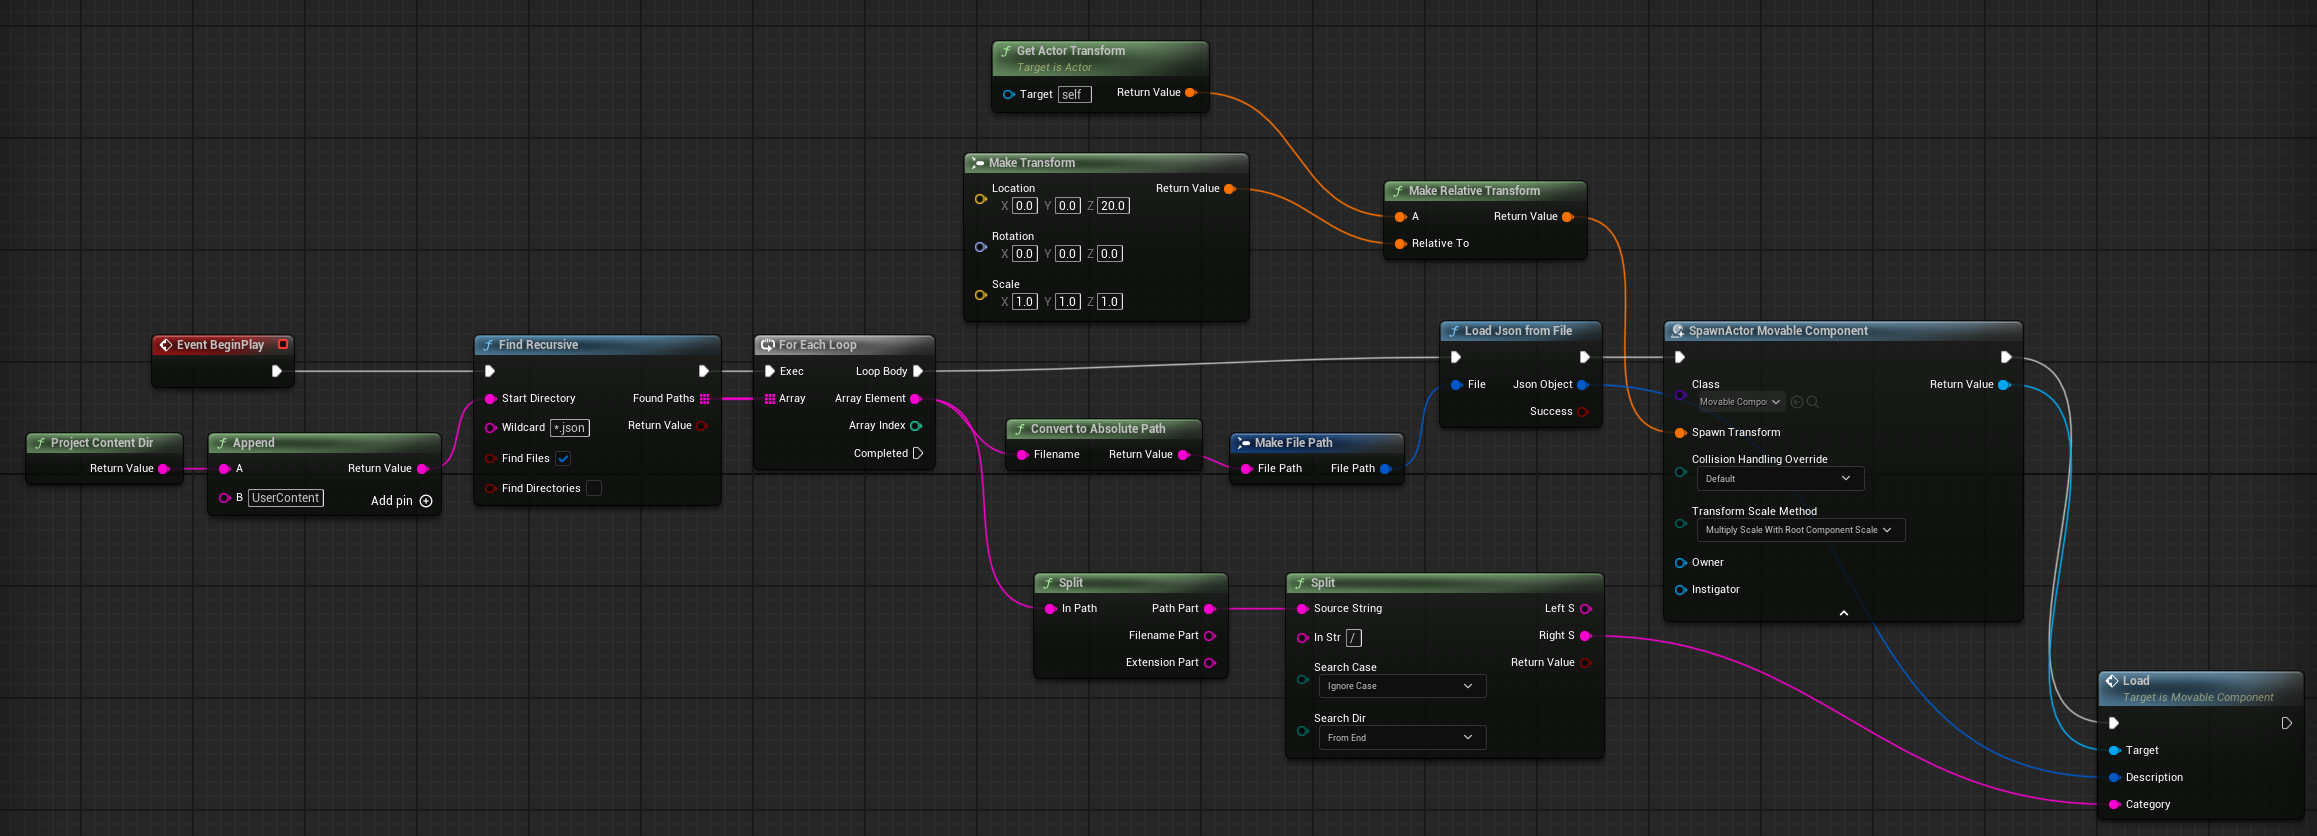
\includegraphics[width=1.0\textwidth]{Images/BasicLoadingBlueprint.png}
% 	\caption{Basic object loading blueprint}
% 	\label{fig:BasicLoadingBlueprint}
% \end{figure}

% The current loading scheme supports loading multiple meshes per object, which gives way to more complex models, such as GPUs with fans.
% Each mesh is expected to be a glTF 2.0 \cite{ISOIEC12113} model file, which is a modern format for 3D models, supporting PBR materials and animations.
% Each mesh can also be assigned a type, which is then used to assign specific functionality to it.
% For example, a mesh of type "Body" is treated as the main mesh of the object, while a mesh of type "Fan" could be rotated when the computer is turned on.

% \begin{figure}[H]
% 	\centering
% 		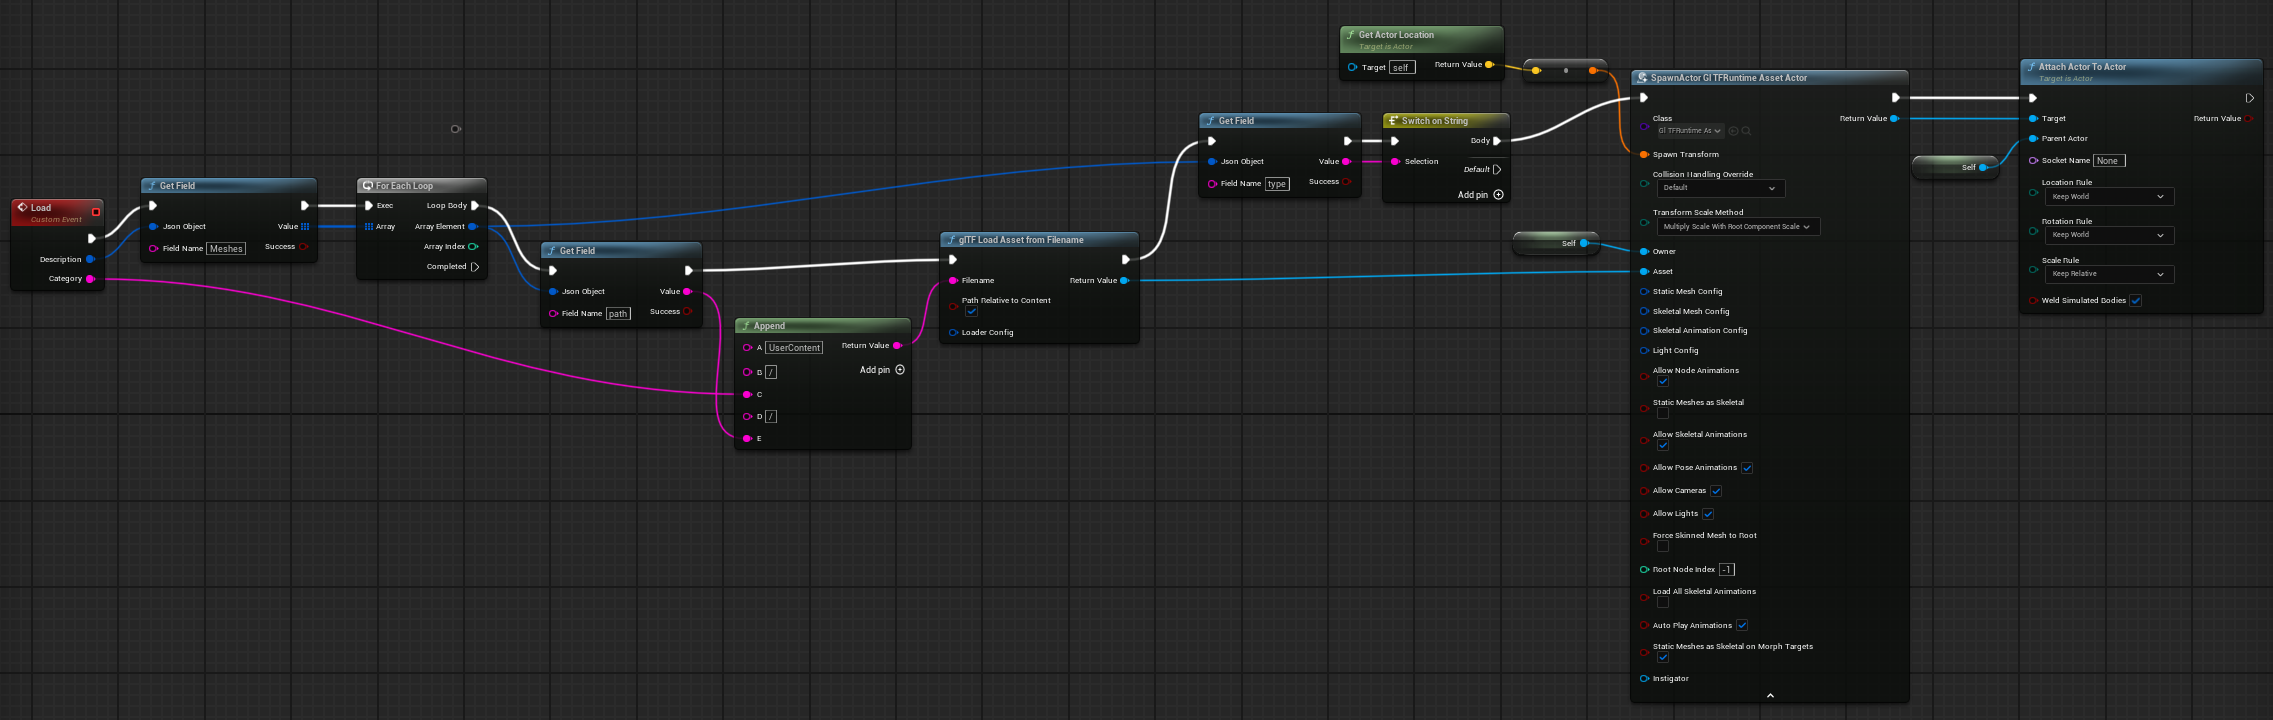
\includegraphics[width=1.0\textwidth]{Images/BasicObjectSelfPreparation.png}
% 	\caption{Basic object self-preparation blueprint}
% 	\label{fig:BasicObjectSelfPreparation}
% \end{figure}

% After placing this loading object in the scene and preparing appropriate description and model files, the object could be spawned in the scene at runtime.

% \begin{figure}[H]
% 	\centering
% 		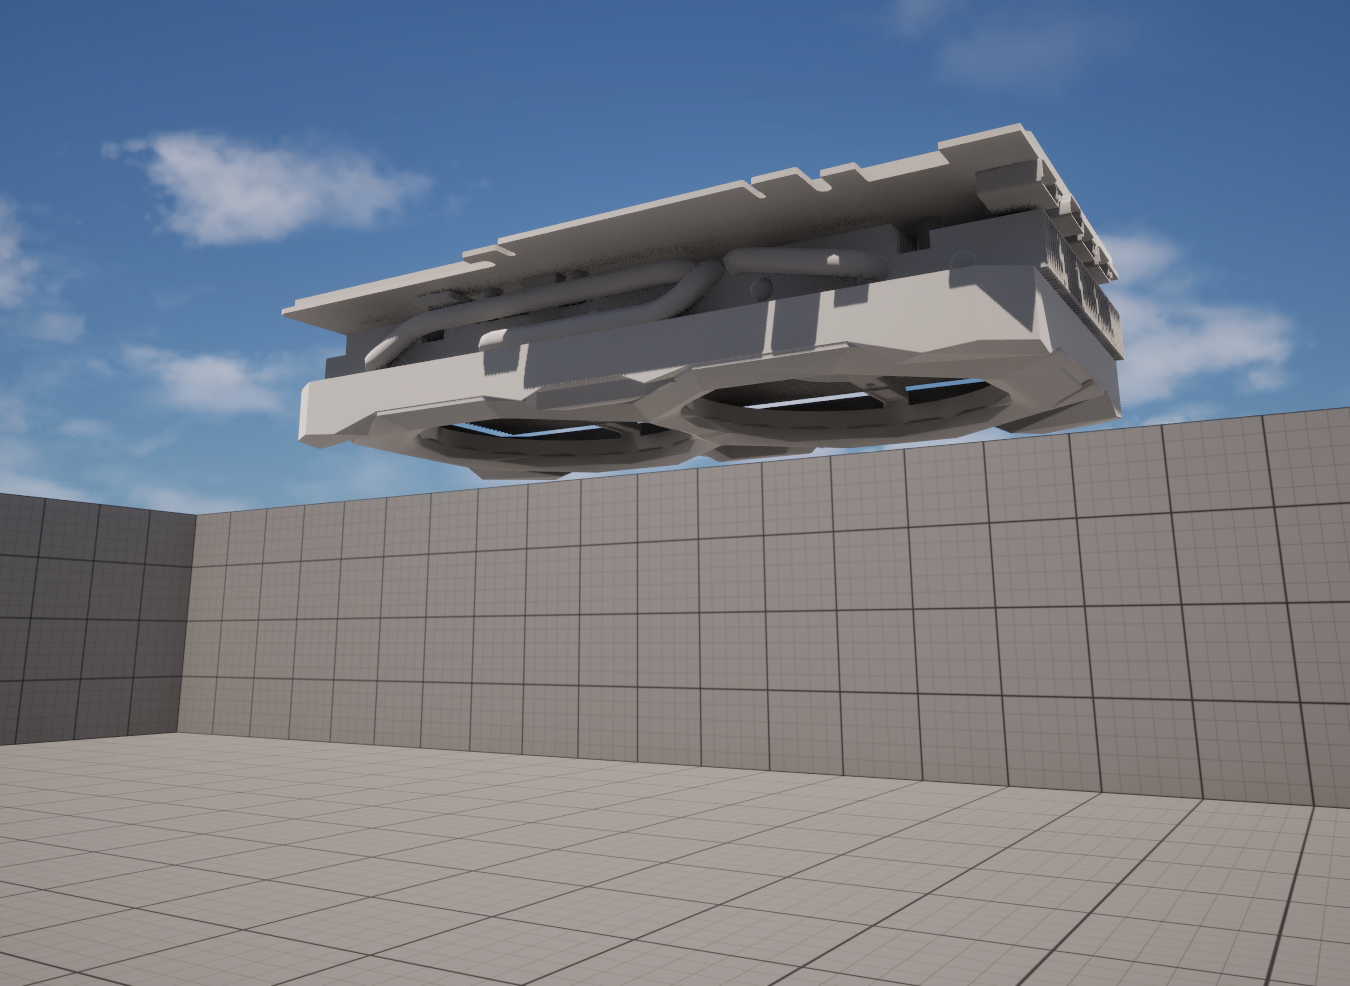
\includegraphics[width=0.7\textwidth]{Images/BasicGPULoaded.png}
% 	\caption{Basic GPU loaded blueprint}
% 	\label{fig:BasicGPULoaded}
% \end{figure}

\subsection{Wider Component Variety (Jakub Jędrzejczyk)}

\subsection{User Settings (Jakub Jędrzejczyk)}

\subsection{Detailed Interactions (Jakub Jędrzejczyk)}

While the current implementation of object interactions in the application is functional and allows users to complete the tasks at hand, there is room for improvement in terms of detail and realism.
Connecting components currently involves simply bringing them close enough to their respective slots, and letting go, at which point they snap into place.

To enhance the realism and immersion of the experience, more detailed interactions could be implemented.
For example, before installing a CPU into its socket, the user would be required to lift the socket lever, remove the protective cover, at which point they could place the CPU into the socket, ensuring it is properly aligned with the notches.
Once in place, the user would then need to lower the lever back down to secure the CPU, otherwise it could fall out during subsequent interactions, nullifying the installation.

Analogously, disconnecting components currently requires pressing a button, then picking up an object, which removes the connection.
A more detailed version of this interaction could involve the user needing to first lift a retention clip or unscrew screws securing the component in place, before being able to safely remove it.

Ideally, together with these features the screws and screwdriver which exist within the game should be fully functional, allowing users to screw and unscrew components as they would in real life.

% bibliografia
% ieeetr - etykiety numerowane w kolejności wystąpienia w tekście
% \bibliographystyle{ieeetr}
% \bibliography{Chapters/Bibliography}
\printbibliography

% wykazy 
\listoffigures
\listoftables

\end{document}
